% paper.tex -- generated by make_tex_v03 from MANUSCRIPT_DRAFT_v06h.md
% manuscript SHA-256 953c210f2fd31daeb5a20c0e06c89d3c9b78fe3e536e4df181d7a9dd0798d954
% bibliography: refs.bib (106 cited entries copied verbatim from refs_v06c_v02.bib)
% Class: ieeeaccess.cls from the IEEE Access LaTeX template (ACCESS_latex_template_20260513); not included here.
% Compile: pdflatex paper; bibtex paper; pdflatex paper; pdflatex paper.  NOT COMPILED BY THE CONVERTER.
% Placeholders to fill before submission are marked \textbf{[...]}; see README_LATEX_v03.md.
\documentclass{ieeeaccess}
\usepackage{cite}
\usepackage{amsmath,amssymb,amsfonts}
\usepackage{algorithmic}
\usepackage{algorithm}
\usepackage{graphicx}
\usepackage{textcomp}
\usepackage{array}
\usepackage{url}
\usepackage{supertabular}

\usepackage{bm}
\makeatletter
\AtBeginDocument{\DeclareMathVersion{bold}
\SetSymbolFont{operators}{bold}{T1}{times}{b}{n}
\SetSymbolFont{NewLetters}{bold}{T1}{times}{b}{it}
\SetMathAlphabet{\mathrm}{bold}{T1}{times}{b}{n}
\SetMathAlphabet{\mathit}{bold}{T1}{times}{b}{it}
\SetMathAlphabet{\mathbf}{bold}{T1}{times}{b}{n}
\SetMathAlphabet{\mathtt}{bold}{OT1}{pcr}{b}{n}
\SetSymbolFont{symbols}{bold}{OMS}{cmsy}{b}{n}
\renewcommand\boldmath{\@nomath\boldmath\mathversion{bold}}}
\makeatother

\def\BibTeX{{\rm B\kern-.05em{\sc i\kern-.025em b}\kern-.08em
    T\kern-.1667em\lower.7ex\hbox{E}\kern-.125emX}}

% --- conversion macros -------------------------------------------------------------------------------
% ragged-right paragraph column for tables
\newcolumntype{L}[1]{>{\raggedright\arraybackslash}p{#1}}
% Tables use the class's native Arabic numbering (TABLE 1 ... TABLE 10); the text cites them as Table 1 ... 10
% (the manuscript's Roman "Table I" ... "Table X" were converted by make_tex_v03).
% algorithm comments print as "# comment", as in the manuscript's pseudocode
\renewcommand{\algorithmiccomment}[1]{\hfill\#~#1}
\newcommand{\AlgInd}{\hspace*{1.2em}}

\begin{document}
% \history and \doi: the IEEE Access template's own placeholders, filled in by IEEE at publication.
\history{Date of publication xxxx 00, 0000, date of current version xxxx 00, 0000.}
\doi{10.1109/ACCESS.2024.0429000}

\title{Planner-Matched Calibration of Tracker Covariances for Chance-Constrained Planning, with a Registered Open-Loop Log-Replay Test on Argoverse 2}
% ---- AUTHOR BLOCK: placeholders; one \uppercase{Name}\authorrefmark{n} per author, \IEEEmembership{...} for members
\author{\uppercase{Ananda Siva Kumar Kopalli Naga Venkata}\authorrefmark{1}}
\address[1]{Independent Researcher (e-mail: anand.knvasks@gmail.com; ORCID: 0009-0002-5241-9922)}
\tfootnote{This work received no external funding.}

\markboth
{A. S. K. Kopalli: Planner-Matched Calibration of Tracker Covariances}
{A. S. K. Kopalli: Planner-Matched Calibration of Tracker Covariances}

\corresp{Corresponding author: Ananda Siva Kumar Kopalli Naga Venkata (e-mail: anand.knvasks@gmail.com).}

\begin{abstract}
Linearized chance-constrained planners need a tracker's covariance to cover the one-sided tail along each constraint normal, which the normalized estimation error squared (NEES) check does not test. On nuScenes, a constant-velocity tracker's 2 s covariance under-covers in-path cars laterally, and NEES-guided inflation of both axes does not fix it. On the constraints a speed planner relies on, the raw covariance is mostly too wide. We propose M$^{*}$, per-stratum conformal risk control fitted on those relied constraints (a proxy at the logged ego trajectory), returned as a covariance for the unchanged planner. In a registered open-loop log-replay test on 375 Argoverse 2 logs with a speed-only planner, M$^{*}$, re-fitted there, was not shown above 5~\% in any evaluable cell on two trackers; its nominal 99.5~\% pooled bounds were at most 0.055, single cells up to 0.16 are not excluded, and it was less often infeasible (forced to back off its designed margin) only than comparators conservative by construction or mostly infeasible. In exploratory analyses after the verdict, with each method tuned to pass a screen on partitions no method stratifies on directly, M$^{*}$ was infeasible in 3--38 percentage points fewer decisions than every comparator family matched within the grid; the smallest gain, against M$^{*}$ without its course-change strata, came with more exceedance at execution on one tracker. M$^{*}$ under-covered low-score and new tracks, failed its screen on a third tracker, and its nuScenes-fitted thresholds did not transfer (in-path pooled exceedance 0.070). Calibration is per constraint, not per decision.
\end{abstract}

\begin{keywords}
Autonomous driving, chance-constrained planning, conformal risk control, covariance calibration, Kalman filtering, multi-object tracking, pre-registration.
\end{keywords}

\titlepgskip=-21pt

\maketitle

\section{Introduction}
\label{sec:introduction}
A chance-constrained motion planner requires each nearby object to stay out of the space the ego vehicle is about to use with probability at least $1 - \delta$ per constraint. Under a Gaussian prediction, a linear constraint becomes a margin $z_{1-\delta}\sqrt{a^{\top}\hat{V}a}$ along its normal $a$~\cite{Blackmore2011,Ono2008}, where $\hat{V}$, for a tracked road user, is a Kalman-filter covariance propagated to the planning horizon~\cite{Zhu2019}, a form driving-scale planners keep~\cite{Nair2025,Ren2025}. The planner thus consumes a \emph{one-sided tail quantile} of the covariance, along directions it chooses.

A tracker's covariance is tuned for association and checked, if at all, by the whole-vector normalized estimation error squared (NEES)~\cite{BarShalom2001,Osterburg2026}, whose acceptance neither implies nor is implied by the property the planner needs; a single-scalar correction over-pays when directions need different corrections (Section III). On nuScenes, a constant-velocity tracker's 2 s covariance shows both effects for in-path cars: the lateral tail is exceeded in 15--27~\% of items against a nominal 5~\% (15.4~\% truth-oriented below 20 m to 27.2~\% estimate-oriented at 20--40 m; Section V-B), the longitudinal tail is over-covered, and the NEES-guided scalar inflates both axes, leaving the lateral tail at 13--17~\% and wasting meters longitudinally.

Those in-path lateral cars are 0.4~\% of the constraints a speed planner actually relies on (T1, nuScenes validation split, classes covered by the learned predictor, 2 s), and on the relied constraints as a whole the raw covariance is mostly \emph{too wide}. A calibration meant to serve a planner must therefore be fitted on the planner's own constraints, not on an audit population chosen in advance.

M$^{*}$ (Section IV) is calibrated on the constraints a chance-constrained speed planner enforces and relies on, a proxy population defined with the logged ego trajectory. It scores the one-sided error along each separating object axis, fits one conformal-risk-control threshold per stratum of features the planner observes, with a count-based fallback and the log as the exchangeable unit, and returns a covariance the planner uses unchanged.

\textbf{The registered claim.} M$^{*}$ and every rule of its test were developed on nuScenes (Section V-C) and then tested in a registered one-shot test on 375 Argoverse 2 logs not used to train the detector, in open-loop log replay with a speed-only planner, its plan frozen before any outcome existed (Section V-D). \textbf{The verdict was GO:} re-fitted within Argoverse 2, M$^{*}$ was not shown above $\delta = 0.05$ in any evaluable cell of the relied constraints on either registered tracker, and its nominal 99.5~\% pooled upper bounds were at most 0.055. But the comparison the registered rule retained was uninformative, since only comparators conservative by construction, or infeasible (forced to back their designed margin off) in most decisions, remained; single cells up to about 0.16 cannot be excluded by the registered bounds, and up to about 0.19 by a better-calibrated interval (Section V-E(c)); M$^{*}$'s thresholds fitted on nuScenes did not carry over to Argoverse 2 (pooled in-path exceedance 0.070, upper bound 0.089, flagged mainly in longitudinal cells; H4); and on a third tracker, AB3DMOT, M$^{*}$ did not pass its screen.

\textbf{Exploratory evidence, added after the verdict} (Section V-E), is not registered: it was specified after reading the registered outputs, in a plan whose hash we recorded ourselves and five amendments. Each comparator family's level, and M$^{*}$'s own, was tuned until it passed a screen on partitions that no method stratifies on directly (M$^{*}$ itself had to drop from $\delta' = 0.05$ to 0.03). M$^{*}$ was then infeasible, that is, had to back off its designed margin, in fewer decisions than every comparator family matched within the grid: by 8--38 percentage points on seven such partitions, and by 3--36 points when track speed and track age, which are related to M$^{*}$'s strata, are removed. The smallest gain, 3--4 points on that reduced screen, is against M$^{*}$ without its course-change strata, and there M$^{*}$ leaves more constraints exceeded at execution on one tracker (T3, +0.054 [0.043, 0.066] on the neutral screen); against the other families, exceedance at execution was similar. A fourth family, the conformal norm ball, still passes at the least conservative level we tried in most folds, so its larger gap is not a matched comparison. One-step progress differed by less than 0.02. M$^{*}$ therefore keeps the planner on its designed margin more often; we do not claim that it makes the planner safer. M$^{*}$ under-covers low-score and newly started tracks, up to about 0.09, an exploratory finding without family-wise control. Throughout, $\delta = 0.05$ is a calibration level per relied constraint, not a safety target, and about half of all decisions keep some exceeded constraint (Section VI-C).

\textbf{Contributions:} (1) a \emph{formal motivation} with elementary results: what a half-space chance-constrained planner consumes from a tracker's covariance, why NEES does not test it, and the price of single-scalar corrections (Section III); (2) \emph{planner-matched calibration,} M$^{*}$ (Section IV); (3) \emph{a registered external test} in log replay on two trackers, with every pre-specified negative (Section V-D); and (4) \emph{exploratory evidence} on what the calibration buys at matched validity and where it fails (Section V-E). Section II positions the work, and Section VI collects its limitations and what is not claimed.

\section{Related Work}
\subsection{Chance-constrained planning with uncertain obstacles}
Under Gaussian uncertainty, chance-constrained control turns a linear constraint's violation probability into a margin along its normal, with risk allocated across constraints or fixed per constraint~\cite{Blackmore2011,Ono2008}, also for Kalman-tracked moving obstacles with the collision region linearized to a half-space~\cite{Zhu2019}. Probabilistic collision checking and planning over uncertain obstacle predictions are treated in~\cite{DuToit2011,Hardy2013}. Driving-scale planners keep affine chance constraints under Gaussian-mixture predictions, tightened per mode by a quantile times a standard deviation~\cite{Nair2025,Ren2025}, or use scenario- or risk-allocating MPC~\cite{deGroot2025,Mustafa2023}; others tighten the same constraints by a conformal radius~\cite{Lindemann2023}, enforce a Mahalanobis keep-out on the whole covariance~\cite{Shah2026,Mohamed2025,Pouria2026}, consume perception uncertainty through chance constraints~\cite{Li2024} or cost weights~\cite{Shi2026}, or bound prediction uncertainty with reachable sets~\cite{Guo2025}. Whether the covariance supports the quantile the planner consumes is assumed, not tested.

\subsection{Where the covariance comes from}
Lidar 3-D multi-object tracking on nuScenes is dominated by Kalman-filter tracking-by-detection~\cite{Weng2020,Chiu2020,Li2023,Osterburg2026}, with noise covariances fitted from training residuals~\cite{Chiu2020}, tuned on tracking metrics~\cite{Osterburg2026}, estimated from innovations in batch~\cite{Mehra1970,Zhang2020} or online~\cite{Sarkka2009,Huang2018,Jiang2024}, or learned or scaled by detection confidence~\cite{Ulreich2024,LearnTrack2026}. Detector-side uncertainty is estimated~\cite{Feng2018,Meyer2020,Pan2020} but not passed to a tracker. Of the nuScenes tracker papers we found, only~\cite{Osterburg2026} reports a consistency statistic for its output covariance, and none certifies the extrapolated covariance a planner consumes.

\subsection{The limits of constant-velocity extrapolation}
Constant-velocity extrapolation is known in motion prediction to be biased on turning vehicles, which motivates turn-rate models, multiple-model filters~\cite{BlomBarShalom1988,Mazor1998,BarthFranke2010} and learned predictors~\cite{Djuric2020,PhanMinh2020} (survey:~\cite{Lefevre2014}), into which a tracker's state uncertainty can be propagated~\cite{Ivanovic2022}; learned models reduce cross-track error severalfold~\cite{Djuric2020}.

\subsection{Assessing covariance consistency}
The NEES/ANEES and NIS $\chi^{2}$ tests~\cite{BarShalom2001} penalize optimism and pessimism asymmetrically and depend on Gaussianity~\cite{Li2002}, hold only for tuned filters~\cite{Chen2024}, fail for mixture filters~\cite{Ahmed2024} and do not separate bias from scale~\cite{Yan2026}; a scalar test can pass while the whitened covariance is wrong~\cite{Forsling2025}, and NEES-based auto-tuning optimizes the whole-vector statistic~\cite{Chen2018nees}. Forecast verification distinguishes calibration notions that do not imply one another~\cite{Gneiting2007}, proposes directional checks~\cite{Ziegel2014} and makes calibration specific to the functional being forecast~\cite{GneitingResin2023}.

\subsection{Conformal prediction and risk control}
Conformal prediction gives finite-sample marginal coverage under exchangeability, per category in its Mondrian form~\cite{Vovk2012,Bostrom2020}, with conditional guarantees over richer covariate classes~\cite{Gibbs2025}; object-conditional validity is impossible in general~\cite{Vovk2012,Lei2014,Barber2021}. Conformal risk control extends it to bounded monotone losses~\cite{Angelopoulos2024,Bates2021}. Scarce classes can be pooled by clustering~\cite{Ding2023}, hierarchical data handled by subsampling one observation per group~\cite{Dunn2023} or by a hierarchical form of exchangeability~\cite{LeeBarberWillett2026}, and thresholds updated online~\cite{GibbsCandes2021}. Training-conditional coverage holds for split conformal but can fail for full conformal and jackknife+~\cite{BianBarber2023}; high-probability variants bound the risk of one fitted rule~\cite{Bates2021,Angelopoulos2025LTT}. Under distribution shift, coverage needs reweighting or degrades~\cite{Tibshirani2019,Barber2023}. Items selected after seeing the data need selection-aware methods~\cite{JinCandes2023,Bao2024}, which our relied-axis scoring does not have. In robotics, conformal regions around predicted trajectories drive MPC~\cite{Lindemann2023,Dixit2023,Lindemann2025}, less conservatively over multiple steps in~\cite{Cleaveland2024}; conformal perception error feeds downstream planners and controllers~\cite{Yang2023,Zhang2025,DixitMei2024}, conformal sets tighten state and input constraints~\cite{Natraj2026,Vlahakis2024}, and~\cite{Su2024} conformalize detection noise inside a tracker.

\subsection{The closest methods, and what is new}
CGKF and CQKF~\cite{Weisman2026} certify joint coverage of a \emph{filtered} state: CGKF by one conformal offset to a Kalman filter's $\chi^{2}$ ellipsoid per time step, CQKF by one shared correction over learned quantiles along 128 random directions, with a one-sided score per direction; both are demonstrated on simulated systems without a planner. LUCCa~\cite{Marques2026a} scales a robot's one-step dynamics covariance by one Mahalanobis-score factor per learned partition for a sampling-based planner, arguing that one global factor is too coarse, which OCULAR~\cite{Marques2026b} shows in simulation. Polyhedral conformal sets~\cite{Chen2026} learn half-space orientations for a robust objective and share one radius; F-CROMS~\cite{Bao2026} selects among score models; conformal tube tightening~\cite{DSilva2026} tightens every polytopic constraint row by one conformal ellipsoidal tube radius. We instead control, per planner-observable stratum, the one-sided tail of a driving tracker's exported Gaussian along each constraint normal that a chance-constrained planner enforces and relies on, and replay the recalibrated covariance into that planner on real logs. None of the works we read does this; the conformal machinery itself is standard.

\subsection{Decision-aware calibration and evaluation}
Decision calibration asks that predictions be calibrated for the decisions made from them~\cite{Zhao2021,Sahoo2021,Kiyani2026,Tang2026,Noarov2025}, and action-conditional guarantees condition on the chosen action~\cite{Zhu2026}. Conformal decision theory~\cite{Lekeufack2024} calibrates the decision itself, controlling a decision loss online; M$^{*}$ instead calibrates offline the covariance a fixed planner consumes. Planner-centric metrics and objectives weigh detection, forecasting or training by their effect on a planner~\cite{Philion2020,IvanovicPavone2022,McAllister2022}; a better-calibrated predictor changed open-loop chance-constrained plans little on real driving data~\cite{IvanovicA2024}. nuPlan defines closed-loop non-reactive and reactive scores~\cite{Karnchanachari2024}. With ground-truth perception,~\cite{Shah2026} evaluate calibrated predictors in a chance-constrained MPC; in pedestrian replay,~\cite{Pouria2026} show that calibration, not displacement error, drives MPC success. Open-loop scores at logged states can disagree with closed-loop behavior~\cite{Dauner2023,Karnchanachari2024} and can be matched from ego status alone~\cite{Li2024Ego}. Demonstrating safety statistically needs far more driving than any study here~\cite{KalraPaddock2016}. Every nuPlan study we found uses ground-truth or noise-injected perception, not a real tracker's recorded covariance.

\section{Formal Motivation}
The statements below are elementary, each with ingredients in print~\cite{Gneiting2007,Ziegel2014,Forsling2025}; they motivate the method but are not its guarantee (Section III-E). Theorem 1(b) and Propositions 3 and 4 are proved in Appendix A, the others in Supplement S8.

\subsection{Setting}
\textbf{(M1) The planner's information.} At decision step $k$ the planner holds $I_{k}$: the tracker's means $\hat{\mu}_{i}$ and position--velocity covariances $\hat{\Sigma}_{i} \succ 0$, with class, size and yaw, and the ego state. A predictor gives mean $\hat{m}_{i}(t)$ and covariance $\hat{V}_{i}(t)$ at horizon $t$. For constant velocity (CV): $\hat{m}_{i}(t) = F_{t}\hat{\mu}_{i}$ and $\hat{V}_{i}(t) = F_{t}\hat{\Sigma}_{i}F_{t}^{\top} + Q(t)$, with $F_{t} = [I_{2}, tI_{2}]$.

\textbf{(M2) The constraints.} For each evaluated tuple $j =$ (candidate plan, object, horizon), the planner forms a unit normal $a_{j}$, offset $b_{j}$ and multiplier $c_{j}$, and checks

\begin{equation*}
a_j^{\top}\hat{m}_j + c_j\sqrt{\hat{v}_j} \leq b_j, \qquad \hat{v}_j = a_j^{\top}\hat{V}_j a_j,\tag{TC}
\end{equation*}
with $c_{j} = z_{1-\delta}$ for a fixed per-constraint risk.

\textbf{(M3) The scores.} With $X_{j}$ the realized position, $U_{j} = a_{j}^{\top}(X_{j} - \hat{m}_{j})/\sqrt{\hat{v}_{j}}$ is the projected standardized error, $N_{j} = (X_{j} - \hat{m}_{j})^{\top}\hat{V}_{j}^{-1}(X_{j} - \hat{m}_{j})$ the NEES, and $\tau_{j} = (b_{j} - a_{j}^{\top}\hat{m}_{j})/\sqrt{\hat{v}_{j}}$ the realized threshold, with $\tau_{j} \geq c_{j}$ when (TC) holds. The guarantee in (TC) is per step, per constraint and open loop.

\subsection{What a half-space planner consumes}
\textbf{Remark 1 (Gaussian half-space reduction).} If $Y \sim N(m, V), V \succ 0$ and $a \neq 0$, then $P(a^{\top}Y > b) \leq \delta$ iff $a^{\top}m + z_{1-\delta}\sqrt{a^{\top}Va} \leq b$.

It underlies the planners of Section II-A~\cite{Blackmore2011,Ono2008,Zhu2019,Nair2025,Ren2025}. The planner's premise is that $a_{j}^{\top}\hat{m} + z_{1-\delta}\sqrt{a_{j}^{\top}\hat{V}a_{j}}$ is a valid $(1 - \delta)$-quantile of the true projected position, \emph{for the normals the planner uses}; we ask whether a tracker's $\hat{V}$ supports it.

\textbf{Definition 1 (decision-projected calibration).} For an $I_{k}$-measurable rule forming constraint instances, $\hat{V}$ is \emph{decision-projected calibrated at level $\delta$} if $P(U_{j} > z_{1-\delta} \mid I_{k}) \leq \delta$ almost surely for every instance. For an $I_{k}$-measurable selection $G$ with $I_{k}$-measurable instance weights, the \emph{stratum form} is $P(U > z_{1-\delta} \mid G) \leq \delta$. This is decision calibration~\cite{Zhao2021} for the loss class $\{1(a_{j}^{\top}y > b_{j})\}$.

\textbf{Proposition 1 (premise).} (i) For an executed plan satisfying (TC), $P(a_{j}^{\top}X_{j} > b_{j} \mid I_{k}) = P(U_{j} > \tau_{j} \mid I_{k})$, so the premise $P(U_{j} > c_{j} \mid I_{k}) \leq \delta$ is sufficient for the per-constraint guarantee, and necessary only on active constraints. (ii) The stratum form is necessary for the premise, but not sufficient in general: a fair label splitting $U \sim N(0, 1)$ into $|N(0, 1)|$ and $-|N(0, 1)|$ gives 0.01 marginally and 0.02 on one label at $z_{0.99}$.

\subsection{Why NEES does not test it}
\textbf{Proposition 2 (plan-uniform criterion).} $(a^{\top}e)^{2}/(a^{\top}\hat{V}a) \leq e^{\top}\hat{V}^{-1}e$ for every $a \neq 0$. Hence $P(N > c^{2} \mid I_{k}) \leq \delta$ implies $P(U > c \mid I_{k}) \leq \delta$ for every $I_{k}$-measurable direction.

Certifying through $N$ costs a margin ratio of 1.30 in two dimensions at $\delta = 0.01$ under Gaussian truth. It is the matched criterion for Mahalanobis keep-out planners~\cite{Shah2026,Mohamed2025,Pouria2026}; a half-space planner needs less.

\textbf{Theorem 1 (NEES and the premise do not imply each other).} At $\delta = 0.01$:

\begin{itemize}
\item \textbf{(a)} Truth $N(0, I)$ and export $\mathrm{diag}(2, 2/3)$ give $E[N] = 2$, exactly consistent in mean, yet the risk along the second axis is 0.0288.
\item \textbf{(c)} Truth $\mathrm{diag}(1, 4)$ and export $I_{2}$ give a calibrated binding direction $e_{1}$, yet $E[N] = 5$. Matching the average NEES globally $(\times2.5)$ leaves a risk of 0.00012 along $e_{1}$, where 0.01 was required.
\end{itemize}

Case (b), a whole-vector $\chi^{2}$ test passed exactly while some direction is above $\delta$, is stated and proved in Appendix A, and case (d), heavy tails, in Supplement S8. Case (c) is the pattern of Section V-B.

\subsection{The price of a single scalar}
Where directions need different corrections, any single multiplier or variance factor fixing the worst direction over-pays elsewhere, by an excess computable per tuple (S8-Proposition 5 and S8-Theorem 2): with lateral and longitudinal constraints, the smallest variance factor bringing the lateral tail to $\delta$ wastes longitudinal margin (the ``price'' of Section V-B). The claim is that one knob over-pays where needs differ, not that no scalar fixes the lateral tail.

\subsection{What this section licenses}
Proposition 1 is conditional on $I_{k}$ and per constraint. Section IV instead certifies a marginal, per-stratum exceedance rate weighting each \textbf{log} equally, on a proxy calibration population (Section IV-G). Such a rate is not measurable at an instance's information and neither implies nor is implied by the premise: under exact conditional calibration it can exceed $\delta$ (0.0625 at $\delta = 0.05$ in an exact example, Supplement S8.2). The formal results therefore motivate \emph{what} to calibrate, one-sided tails along the planner's constraint normals, stratified by what it observes; Sections V-C to V-E test it empirically.

\section{Method: Planner-Matched Calibration (M$^{*}$)}
M$^{*}$ is a post-processor between tracker and planner (Fig.~1), fitted offline on logs with ground truth and deployed online as a recalibrated covariance that the planner consumes unchanged. Its parts are published: conformal risk control (CRC)~\cite{Angelopoulos2024}, Mondrian, per-category validity~\cite{Vovk2012}, one score per exchangeable unit~\cite{Dunn2023} and conformal inflation of a Kalman-filter confidence region~\cite{Weisman2026} and of a dynamics covariance consumed by a planner~\cite{Marques2026a}. \textbf{What M$^{*}$ adds} is the \textbf{calibration population}, the constraints a chance-constrained planner actually enforces and relies on, rather than a fixed audit population, with \textbf{scoring in constraint coordinates} (IV-A); \textbf{strata} the planner observes, with a count-based fallback (IV-B, IV-D); and a \textbf{deployable covariance} that reproduces the calibrated margins exactly (IV-E). M$^{*}$ grew out of DP-SCRC, the same machinery fitted on a fixed in-path audit population; a pre-specified planner study found that the planner relied on constraints outside that population, where DP-SCRC was significantly above $\delta$ (Supplement S1--S2).

\begin{figure}[!t]
\centering
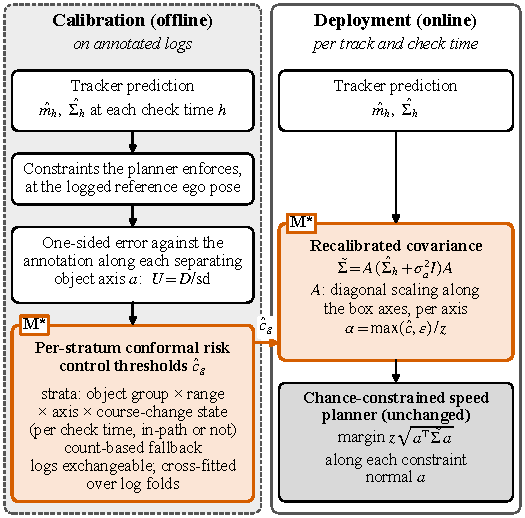
\includegraphics[width=\columnwidth]{figs/fig01_pipeline.pdf}
\caption{M$^{*}$ between tracker and planner. Offline (left), on annotated logs, each constraint the planner enforces at the logged reference ego pose gives a one-sided error $U = D/\mathrm{sd}$ of the tracker's prediction along each separating object axis. Conformal risk control then sets one threshold $\hat{c}_g$ per stratum (object group $\times$ range $\times$ axis $\times$ course-change state, fitted separately per check time and for in-path and other tracks), with a count-based fallback to coarser cells, the log as the exchangeable unit and cross-fitting over log folds. Online (right), the thresholds rescale the tracker's covariance along the box axes, $\tilde{\Sigma} = A(\hat{\Sigma}_h + \sigma_a^2 I)A$ with $\alpha = \max(\hat{c}, \varepsilon)/z$ per axis, and the unchanged chance-constrained speed planner applies its usual margin $z\sqrt{a^{\mathsf{T}}\tilde{\Sigma}a}$, which equals $\hat{c}\cdot\mathrm{sd}$ along each object axis (Proposition 5).}
\label{fig:1}
\end{figure}

\subsection{The calibration population}
The planner is the chance-constrained speed planner of Appendix B (Section V-A). For a track and one of its two box axes $a$ (longitudinal $a_{L}$ or lateral $a_{T}$, from the estimated yaw), the \emph{gap} at a check time is the clearance along $a$ between the buffered ego footprint and the object's box; a (track, check time) pair is safe under a margin $m$ if some axis has gap $\geq m$. A pair is \emph{enforced} if, at the arm-independent reference margin 0, some candidate plan satisfies it and so would an ego held at its current position (a conflict the other agent brings to a stopped ego is not the planner's to resolve). Only tracks with a detection score $\geq 0.4$, within 60 m and not behind the ego count.

\textbf{Items.} At every decision state of a log (every keyframe but the first and the last, at the logged ego's position and speed) and every calibrated check time $h \in \{0.5, 1, 1.5, 2\}$ s, each enforced pair whose object has an annotation at $k + h$ ($\geq 1$ lidar point, not inside a bicycle rack) gives one item per object axis that separates the pair at the \textbf{reference ego pose}:

\begin{equation*}
D = s\cdot a^{\top}(X - \hat{m}), \qquad \mathrm{sd} = \sqrt{a^{\top}\hat{\Sigma}_h a + \sigma_a^2}, \qquad U = D/\mathrm{sd},
\end{equation*}
with $s$ the side of separation (positive $D$: the object came closer than predicted), $\hat{m}$ and $\hat{\Sigma}_{h}$ the tracker's predicted mean and $2 \times 2$ covariance at $h$, $X$ the annotated center and $\sigma_{a} = 0.10$ m an assumed annotation noise. A margin $m$ along $a$ is \emph{exceeded} when $D > m$.

\textbf{The relied axis and the scored populations.} Fitting uses every separating axis of every enforced pair at the reference pose. Scoring (Section V) uses, per enforced pair, the \emph{relied axis} under \textbf{each arm's own chosen plan}: the axis with the largest slack (gap minus that arm's margin), kept if it separates (gap $> 0$) and the plan satisfies it at the arm's full margin. $P_{\mathrm{rel}}$ holds all such records, $P_{\mathrm{near}}$ those with pair gap $\leq 5$ m, $P_{\mathrm{ip}}$ those of in-path tracks and $P_{\mathrm{nip}}$ those of other tracks (scope only). The scored sets therefore differ between arms: on Argoverse 2 T1, $P_{\mathrm{rel}}$ holds 534,846 records under M$^{*}$ and 356,260 under B3, against 537,924 relied items at the reference pose (Supplement S9.11).

\textbf{The reference pose: a proxy.} Fitting needs a reference ego progression before any arm has chosen a plan; M$^{*}$ uses the \textbf{logged} ego pose at $t_{k} + h$, which a driver chose knowing the true object positions, so the calibration population is a proxy defined with the logged ego trajectory (Section IV-G; Section V-E(d) refits M$^{*}$ at two references that use nothing after $t_{k}$).

\subsection{Strata}
The strata use features the planner observes at decision time: \textbf{group} (car; pedestrian; two-wheeler; large vehicle); \textbf{range} of the predicted object from the ego's constant-turn-rate-and-velocity (CTRV) predicted center at $k + h$ ($< 20$ m, 20--40 m, $\geq 40$ m); \textbf{axis} (longitudinal or lateral); and \textbf{course-change state,} from the track's own exported positions: \emph{static} if speed $< 1.0$ m/s, otherwise \emph{new} if the turn rate is undefined, otherwise \emph{turning} if $|\hat{\omega}| \geq 0.10$ rad/s, otherwise \emph{straight}. Level 0 has $4 \times 3 \times 2 \times 4 = 96$ strata; the coarser levels are L1 $=$ group $\times$ range $\times$ axis, L2 $=$ group $\times$ axis and L3 $=$ axis. Fitted separately per check time and for in-path and other tracks, M$^{*}$ has 192 thresholds per check time. The taxonomy is fixed in advance; no partition is learned.

\subsection{Per-stratum conformal risk control, with the log as the unit}
\textbf{The exchangeable unit} on Argoverse 2 is the log, in fitting, cross-fitting and the bootstrap. The nuScenes development fits used the 20 s scene; scenes cut from one drive are dependent, so there Proposition 3 holds only as far as scenes are exchangeable, and an exact example shows it can fail ($2/31 = 0.0645$ at $\delta = 0.05$; S8-Remark A.5), one reason the nuScenes evidence is development evidence (its bootstraps resample whole drives).

For stratum $g$ and threshold $c$, the \emph{log loss} $L_{g}(Z; c)$ is the share of log $Z$'s items in $g$ with $U > c$: non-increasing and right-continuous in $c$, in [0, 1], and 0 for $c \geq \max U$. With $n$ calibration logs that contain $g$,

\begin{equation*}
\hat{c}_g = \inf\Bigl\{c : \frac{n}{n + 1}\cdot\frac{1}{n}\sum_i L_g(Z_i; c) + \frac{1}{n + 1} \leq \delta\Bigr\},
\end{equation*}
and the deployed margin is $\hat{c}_{g}\cdot\mathrm{sd}$. The rule is evaluated in exact rational arithmetic, so the threshold depends only on the multiset of logs.

\textbf{Proposition 3 (per-stratum validity, log unit; proof in Appendix A).} Let the logs $Z_{1}, \dots, Z_{m}$ and $Z_{\mathrm{test}}$ be i.i.d., the item map (tracker, predictor, strata and reference rule) fixed outside the evaluation logs, and each log contain an item in $g$ with positive probability. If the $N \geq 19$ calibration logs with an item in $g$ are used and $Z_{\mathrm{test}}$ has an item in $g$, then $E[L_{g}(Z_{\mathrm{test}}; \hat{c}_{g}) \mid N] \leq \delta = 0.05$: an item drawn uniformly from the test log's stratum-$g$ items exceeds $\hat{c}_{g}$ with probability at most $\delta$. The same holds for each cross-fitted fold (Appendix A, Corollary A.4).

The bound is marginal over the calibration logs, not a bound for one fitted rule: in a simulation at 300 calibration logs the expected risk is 0.045, but the risk of a single fitted rule exceeds $\delta$ in about a quarter of calibration draws (Appendix A). \textbf{The sample floor:} a finite $\hat{c}_{g}$ needs $N \geq 1/\delta - 1 = 19$ logs, and 99 at $\delta = 0.01$; smaller levels cannot be certified by this construction with fewer logs (S8-Remark 5).

\subsection{Count-based fallback}
A level-0 stratum with fewer than 19 calibration logs takes the threshold of the first coarser cell on its chain L0 $\subset$ L1 $\subset$ L2 $\subset$ L3 with at least 19.

\textbf{Proposition 4 (fallback; proof in Appendix A).} (i) A stratum assigned its own threshold keeps Proposition 3, conditionally on that assignment. (ii) A stratum $g$ assigned a coarser cell $C$'s threshold is covered only through $C$: a test log's share of $C$-items above $\hat{c}_{C}$ has expectation at most $\delta$, given $C$'s membership vector and a test log containing $C$. Nothing is asserted for $g$'s own items, for the deployed loss over $C$, given that the test log contains $g$, or given $g$'s fallback event (an exact counterexample gives 0.0481 for $C$ overall but 0.0536 given that $g$ falls back). (iii) The assignment depends on the data only through counts, so the deployed rule is a fixed map from tracker-observable features to thresholds.

\subsection{The deployable covariance}
\textbf{Proposition 5 (deployable covariance).} For the estimated box axes $a_{l}$ and $a_{t}$ and $\alpha_{l}, \alpha_{t} > 0$, let $A = \alpha_{l}a_{l}a_{l}^{\top} + \alpha_{t}a_{t}a_{t}^{\top}$ and $\tilde{\Sigma} = A(\hat{\Sigma} + \sigma_{a}^{2}I)A$. Then $\tilde{\Sigma} \succ 0$ and $a^{\top}\tilde{\Sigma}a = \alpha^{2}(a^{\top}\hat{\Sigma}a + \sigma_{a}^{2})$ on each axis. With $\alpha = \max(\hat{c}, \varepsilon)/z_{1-\delta}, \varepsilon = 10^{-3}$, a planner applying $z_{1-\delta}\sqrt{a^{\top}\tilde{\Sigma}a}$ applies exactly $\hat{c}\cdot\mathrm{sd}$ (or $\varepsilon\cdot\mathrm{sd}$) along each object axis. A planner normal that is not an object axis receives a mixture of the two corrected axes, which no certificate covers.

\subsection{Algorithm}
Algorithm 1 in Appendix B gives the steps. On Argoverse 2 each of 5 log folds is calibrated on the other 300 logs (cross-fitting).

\subsection{What the theory covers, and what it does not}
No result in this paper bounds exceedance on the scored relied records; that is measured (Section V).

\textbf{Covered.} Within one dataset, cross-fitted M$^{*}$ has Proposition 3's marginal per-stratum bound for its own-threshold strata \emph{on its calibration items}, since logs are exchangeable and the item rule is the same in calibration and test. An exploratory check added after the verdict (amendment A3) agrees on Argoverse 2: on its own calibration items, cross-fitted M$^{*}$ is flagged in none of its 93 (T1) and 92 (T3) evaluable own-threshold strata, with pooled exceedance 0.043 and 0.042, and 0.7~\% of items in fallback strata; of the scored in-path relied records, however, 7.5~\% (T1) and 7.6~\% (T3) fall in fallback strata.

\textbf{Not covered} (Supplement S8.7): \textbf{relied-axis selection} (the scored records are a subset selected by gap, under each arm's own plan); \textbf{the proxy population} (Proposition 1 and S8-Proposition 3 need every ingredient of the constraint to be measurable at $I_{k}$, and the logged reference pose is not); \textbf{pooled and fallback cells} (covered only as in Proposition 4(ii)); \textbf{one deployed rule} (cross-fitting estimates the risk averaged over five fold rules, not a bound for the single rule a deployment would fit on all logs); and \textbf{the premise itself} (Section III-E). The registered test (Section V-D) and the exploratory analyses (Section V-E) check these parts empirically; they do not prove them.

\subsection{Comparators}
All arms are margins along an object axis. \textbf{The registered comparator set $K$} (Section V-D) was fixed on development data: \textbf{B0}, the raw covariance, $1.645\cdot\mathrm{sd}$; \textbf{B1}, NEES-scaled, $k = \mathrm{ANEES}/2$ per group $\times$ range~\cite{BarShalom2001,Osterburg2026}; \textbf{B3}, the largest of M$^{*}$'s thresholds, at least M$^{*}$'s margin on every item; \textbf{B4}, one pooled CRC threshold per check time, the analogue of the per-time-step conformal inflation of~\cite{Weisman2026} and of a single global factor~\cite{Marques2026b}; \textbf{B6}, M$^{*}$ without course-change strata; \textbf{B9}, a norm-ball CRC radius~\cite{Lindemann2023,Dixit2023}; and \textbf{RETUNED}, B0 rescaled to a pooled 5~\% on the training folds. \textbf{Exploratory arms} (RETUNED-HK1, B4, B6 and B9 at stricter levels, B5, B7, B8 and a re-fitted process noise) are defined in Section V-E.

\section{Experiments}
\subsection{Data, stack and planner}
\textbf{Data.}

\begin{itemize}
\item \textbf{Argoverse 2}~\cite{Argoverse2}, the registered test: 375 logs of the Sensor dataset, namely 225 training logs held out from our detector by a seeded permutation and the 150 validation logs. Each log is one drive segment of about 15 s with 3-D annotations, used at 2 Hz.
\item \textbf{nuScenes}~\cite{Caesar2020}, development only: 850 scenes of about 20 s, annotated every 0.5 s and cut from 68 drives; train and validation do not share a drive.
\end{itemize}

\textbf{Detectors.} On Argoverse 2, CenterPoint~\cite{Yin2021} in the LT3D code base~\cite{Peri2022}, trained by us on the other 475 Argoverse 2 training logs with the public configuration, for 2 class-balanced epochs~\cite{Zhu2019cbgs} (set by a compute cap) against the public checkpoint's 20. On nuScenes, a CenterPoint checkpoint trained on nuScenes train, so detections on train are in-sample; its exact checkpoint is not recorded (Supplement S9.15).

\textbf{Trackers} (Table 1): \textbf{T1,} CANMOT~\cite{Osterburg2026}, an extended Kalman filter with a constant-velocity model for every class; \textbf{T3,} Poly-MOT~\cite{Li2023}, as configured in CANMOT's \path{paper/baseline/poly_mot} experiment (the original Poly-MOT uses a bicycle model for bicycles and motorcycles); and \textbf{AB3DMOT}~\cite{Weng2020}, the LT3D implementation with its defaults, a descriptive third tracker on Argoverse 2. All keep their nuScenes noise parameters and run at 2 Hz on Argoverse 2.

\textbf{Extrapolation.} The 2 s covariance is each tracker's own filter prediction repeated over the horizon without measurement updates: a constructed open-loop extrapolation, since the tracker's process noise was tuned for one-step association.

\textbf{Matching.} Tracks are matched to annotations by Hungarian assignment within 2 m; certificates cover matched true positives only (Section VI-F).

\textbf{The planner} (summary and Algorithm 2 in Appendix B; full specification in Supplement S9). The ego follows its logged path and chooses its speed among 32 accelerate-then-brake candidates (some never accelerate, and four are duplicates) and an emergency stop; only the ego's footprint is buffered (0.5 m). Every 0.25 s to 2 s, each tracked object must be kept apart from the ego along some box axis by at least the arm's margin; only \emph{enforced} pairs bind (Section IV-A), and the candidate with the largest mean progress that satisfies every enforced constraint is chosen.

\begin{itemize}
\item \textbf{Infeasible decisions.} If no candidate satisfies them at the arm's full margin, the decision is \emph{infeasible}: the planner backs its designed margin off, to 0.75, 0.5, 0.25 and 0 of its value, and takes the emergency stop only if even the buffered ego and the object's box cannot be kept apart. ``Infeasible'' therefore means ``designed margin backed off'', not ``no progress''.
\item \textbf{Decision mode,} used for every comparison: one open-loop decision per keyframe from the logged ego state, with the plan leashed so that it never gets ahead of the logged ego; every arm is scored on the constraints it relied on under its own chosen plan.
\end{itemize}

\begin{table*}[!t]
\centering
\caption{Trackers.}
\label{tab:1}
\footnotesize
\setlength{\tabcolsep}{4pt}
\renewcommand{\arraystretch}{1.15}
\begin{tabular}{@{}L{0.244\textwidth}L{0.263\textwidth}L{0.292\textwidth}L{0.149\textwidth}@{}}
\hline
Tracker & Motion model & Noise & Tuned on \\
\hline
T1 CANMOT \path{paper/local/canmot/sc} & EKF, constant velocity, $Q$ rotated into the box frame & $Q$ by Bayesian optimization for AMOTA; $R$ the sample covariance & nuScenes validation $(Q)$, trainval $(R)$ \\
T3 Poly-MOT \path{paper/baseline/poly_mot} (CANMOT config) & CTRA EKF for car, bus, pedestrian, truck; linear CA for bicycle, motorcycle, trailer & its own $Q$ and $R$, hand-set (CTRA $Q$ the identity) & association on nuScenes validation \\
AB3DMOT (LT3D) & linear constant velocity, one step per frame & LT3D defaults: $Q$ the identity with 0.01 on velocities; $R$ the filter library's default identity & not re-tuned (set for 10 Hz use) \\
\hline
\end{tabular}
\end{table*}

The nuScenes study also used a second CANMOT setting (T2, data-fitted $Q$) in the method stage (Supplement S1).

\subsection{Motivation: a mis-shaped extrapolated covariance}
\textbf{Design.} A pre-specified study measured the one-sided tail of the error along the toward-ego box axes of in-path cars, at 2 s, under T1, a CANMOT tracker with a constant-velocity model, on the 700 nuScenes training scenes; the predictor is the tracker's own state and covariance extrapolated 2 s. Its plan was frozen with its code before its outcomes were computed (one pre-freeze check previewed the decision; Section VI-D). This is an \emph{audit} population (Supplement S1), not the planner's relied constraints: it shows that the covariance is mis-shaped, and that the standard check sends the correction the wrong way.

\textbf{Results (Table 2).} Laterally, the toward-ego margin is exceeded in 19.4~\% ($< 20$ m) and 27.2~\% (20--40 m) of items, against a nominal 5~\% (estimate-oriented, record-weighted rates; Table 2 also gives scene-weighted ones). \textbf{Truth-oriented,} with the side of the ego taken from the true position so that the orientation artifact is removed, they are 15.4~\% and 22.8~\%. Longitudinally, the margin is exceeded in 0.4~\% and 1.1~\%: the covariance is too wide along the box. The NEES-guided scalar leaves the lateral tail at 13.0~\% and 17.2~\%, and any single variance factor that fixes the lateral tail adds 10--12 m of unneeded longitudinal margin (the ``price'' of Section III-D: 11.61 m and 10.34 m, one-sided 97.5~\% lower bounds 9.81 m and 8.24 m).

\begin{table*}[!t]
\centering
\caption{Decision cells of the nuScenes diagnosis: 2 s extrapolation, in-path cars, nuScenes train, $\sigma_{a} = 0.10$ m; one two-sided 95~\% sup-t band over four cells. $E$ is record-weighted (share of items; with the band and the verdict) or scene-weighted (mean of per-scene shares); Argoverse 2 rates are log-weighted.}
\label{tab:2}
\footnotesize
\setlength{\tabcolsep}{3pt}
\renewcommand{\arraystretch}{1.15}
\begin{tabular}{@{}L{0.193\textwidth}L{0.142\textwidth}L{0.074\textwidth}L{0.142\textwidth}L{0.073\textwidth}L{0.080\textwidth}L{0.081\textwidth}L{0.126\textwidth}@{}}
\hline
Cell & $E$ estimate-oriented, record [band] & $E$ estimate-oriented, scene & $E$ truth-oriented, record [band] & $E$ truth-oriented, scene & Items / scenes (estimate-oriented) & Threshold $\max(0.05, E^{0})$ & Verdict \\
\hline
car $< 20$ m, lateral & \textbf{0.194} [0.152, 0.236] & 0.141 & 0.154 [0.116, 0.193] & 0.098 & 3,396 / 442 & 0.0775 & FAILS \\
car 20--40 m, lateral & \textbf{0.272} [0.205, 0.338] & 0.245 & 0.228 [0.162, 0.293] & 0.175 & 1,229 / 219 & 0.0816 & FAILS \\
car $< 20$ m, longitudinal & 0.004 [0.002, 0.007] & 0.008 & -- & -- & 8,038 / 529 & 0.0646 & OVERCOVERS \\
car 20--40 m, longitudinal & 0.011 [0.004, 0.017] & 0.019 & -- & -- & 3,522 / 345 & 0.050 & OVERCOVERS \\
\hline
\end{tabular}
\end{table*}

\textbf{What ``lateral'' means.} ``Lateral'' is the tracked box's lateral axis, from the tracker's estimated yaw, and CANMOT's box headings are often wrong: in a project audit of the nuScenes planner population, records produced by T1 but not by T3 came mostly from boxes more than 20$^{\circ}$ off the annotation (median 40$^{\circ}$ in the in-path car lateral straight cell), while Poly-MOT's headings were off by a median of about 1$^{\circ}$. A box rotated by 40$^{\circ}$ turns part of the world's longitudinal error into ``lateral'' error. \textbf{In the diagnosis cells,} a post-registration check, specified before it was computed (amendment A1 of the exploratory plan, Section V-E), rebuilt the diagnosis items exactly and measured each item's heading error against its annotation: 35--39~\% of lateral items come from boxes more than 20$^{\circ}$ off, and they carry 41--49~\% of the lateral exceedances. \textbf{Heading error explains part of the failure, not all of it} (amendments A1 and A4; pointwise scene-bootstrap intervals; Supplement S6.10 and S6.20). Restricted to boxes within 5$^{\circ}$ of the annotation, the lateral exceedance is still 0.10--0.23, above every cell's threshold (0.05 truth-oriented; 0.0775 and 0.0816 estimate-oriented, Table 2). Measured along the annotated box's own lateral axis, it stays above its threshold below 20 m (0.124 estimate-oriented, 0.089 truth-oriented), but at 20--40 m the intervals include the thresholds (0.108 [0.074, 0.143] against 0.0816; 0.064 [0.040, 0.093] against 0.05). The longitudinal cells stay at or below 0.02.

\textbf{Scope of the finding.} It is a constant-velocity effect: the extrapolation under-predicts the lateral spread of turning vehicles (Section II-C). Under T3 (Poly-MOT, CTRA for cars) the raw covariance is far too wide rather than mis-shaped (mean lateral margin 32.1 m). What is new is not the under-dispersion itself but its consequence at the tracker--planner interface: the standard NEES check sees the inflated average and recommends inflating every direction, including the already over-covered longitudinal one (Theorem 1(c)).

\textbf{Partial replication on Argoverse 2 (H8, registered).} On T1 under the raw covariance, the 20--40 m lateral cell fails in both versions (0.214 [0.122, 0.306] against $E^{0} = 0.090$, and truth-oriented 0.144 [0.068, 0.220]); the $< 20$ m lateral cell fails only estimate-oriented (0.147) and is consistent truth-oriented (0.088 [0.046, 0.130]); and the 20--40 m longitudinal cell, outside H8's definition, also fails, at 0.158 [0.106, 0.210], which the nuScenes diagnosis did not show. The lateral under-coverage thus replicated where it was largest. The longitudinal over-coverage, and with it the ``price'' of a lateral-fixing scalar, did not replicate at 20--40 m, where both axes under-cover; H8 is therefore a partial replication.

\subsection{Development on nuScenes (exploratory)}
M$^{*}$ and every rule of the registered test were developed on 840 nuScenes scenes (68 drives; the 850 of Section V-A less the 10 nuScenes-mini development scenes): the recorded covariances of T1 and T3 replayed into the planner of Appendix B in decision mode, with fits cross-fitted over 5 scene folds and a drive-cluster bootstrap. This is development evidence, reported in full in Supplement S2.2: the fits use the scenes M$^{*}$ was built on, T1's process noise was tuned on nuScenes validation, and the gates are ours.

M$^{*}$ was not shown above $\delta$ in any cell, power-qualified family or pooled cell of $P_{\mathrm{rel}}, P_{\mathrm{near}}$ or $P_{\mathrm{ip}}$, on either tracker. \textbf{The raw covariance is mostly too wide on this population:} B0's pooled $P_{\mathrm{rel}}$ exceedance is 0.026 (T1) and 0.002 (T3), and the in-path lateral cars of Section V-B are 0.4~\% of relied items on the validation split (T1, classes covered by the learned predictor, 2 s). M$^{*}$ therefore mostly \emph{narrows} margins, recovering feasibility where the raw covariance is too wide while holding the exceedance near $\delta$ where it is too narrow; on T3 the narrower margins cost real violations. \textbf{Per constraint is not per decision:} about one decision in three had some relied constraint exceeded (V2 0.358 and 0.351), 0.04--0.05 above the per-track reference $1 - 0.95^{n_{\mathrm{tracks}}}$, and calibrating one scalar on the union loss (M$^{*}$J) brings V2 to about 0.05, at +0.31 and +0.39 in infeasible-decision rate.

The registered test was designed to check these patterns on new data (the validity of M$^{*}$, how often it backs off its margin compared with the comparators, and the cost of the strata), accepting that the comparators retained by the screen might be only conservative ones (Section V-D).

\subsection{The registered test on Argoverse 2}
\textbf{1. Registration.} The plan was frozen on 6 Nov 2026, 20:08:13 UTC, binding 354 files by hash, and registered on OSF under embargo at 20:31 UTC (\url{https://osf.io/v8qfk/}; reviewers receive a view-only link; Supplement S7 outlines the frozen plan). Reading annotation positions after a decision time requires a deposit record naming the registration, and every guarded run is logged in a hash chain. \textbf{This blinding is procedural, not technical} (Section VI-D): the detector port was checked before the freeze on the 150 validation logs, which are part of the test set.

\textbf{2. Data, detector and trackers} are those of Section V-A (configurations in Supplement S9). Our detector's 26-class AP at 50 m is 0.425 on validation and 0.415 on the held-out logs, against 0.469 for the public checkpoint.

\textbf{3. Design.} M$^{*}$ is re-fitted within Argoverse 2 by 5-fold cross-fitting over logs (Section IV); the comparators $K =$ \{B0, B1, B3, B4, B6, B9, RETUNED\} were fixed on development data. \textbf{The primary claim, H1,} is Form B on both trackers: M$^{*}$ passes the screen and is less often infeasible than every comparator not itself shown above $\delta$ (the comparison set $V_{t}$). The statistical design is explained after this item in plain terms, the terminology table (Appendix C) defines every label, and the secondary claims H2--H10 are listed in Section V-D8. Two properties of this design, stated before the results:

\begin{itemize}
\item \textbf{The comparison set may be uninformative.} B3's margin is at least M$^{*}$'s on every item, and on development the screen retained only B3 (T1) and B0 and B3 (T3).
\item \textbf{The screen's cells are M$^{*}$'s own strata} (group $\times$ axis $\times$ course-change state, pooled over range). B0, B1, B4, B6, B9 and RETUNED, not stratified by course-change state, can pass a course-change cell only by being conservative there, so part of their flags follows from the choice of cells. Section V-E(b) screens every arm on partitions no method stratifies on directly.
\end{itemize}

\textbf{The statistical design of the registered test, in plain terms.}

\emph{What is measured.} For one arm (a margin rule) on one tracker, every relied constraint of every decision gives one record: did the realized error along the relied axis exceed the arm's margin? Records are grouped by population $(P_{\mathrm{rel}}, P_{\mathrm{near}}, P_{\mathrm{ip}})$ and into cells (class group $\times$ axis $\times$ course-change state, pooled over range). A cell's exceedance rate is the mean over logs of each log's share of exceeded records (logs without a record in the cell are skipped); all intervals resample whole logs $(B = 40{,}000)$.

\emph{The screen: three checks on M$^{*}$, per tracker and population.}

\begin{enumerate}
\item[1.] \textbf{No flag.} A cell is \emph{flagged} (``shown above $\delta$'') when the lower end of a one-sided simultaneous 95~\% sup-t log-bootstrap band over all evaluable cells (records from $\geq 39$ logs) lies above $\delta = 0.05$; the same rule applies to the power-qualified family and to the pooled cell.
\item[2.] \textbf{Floors.} $\geq 6$ \emph{power-qualified} cells (a planted rate of 0.15 in the cell alone would be flagged with probability $\geq 0.8$) on $P_{\mathrm{rel}}$ and $P_{\mathrm{near}}$; $\geq 1$ evaluable cell on $P_{\mathrm{ip}}$.
\item[3.] \textbf{HK1c.} The pooled rate's upper bound at nominal 99.5~\% is $\leq \delta + 0.03 = 0.08$: the one check that rejects something.
\end{enumerate}

\emph{Form B, H1 and GO.} H1 spends one-sided 0.025 in two halves. A comparator leaves the comparison set $V_{t}$ only if flagged in any of its 9 conditions at one-sided $1 - 0.0125/9 = 0.99861$ each (the removal half, 0.0125); M$^{*}$ must then be less often infeasible than every member of $V_{t}$, by a paired log-bootstrap bound at one-sided $0.0125/|V_{t}|$ each (the superiority half, 0.0125). \textbf{H1} $=$ Form B on both trackers, an intersection--union test in which every component must reject~\cite{Berger1982}; \textbf{GO} $=$ H1 with every input present and of verified provenance.

\textbf{What GO controls, and what it does not.} A pooled exceedance above 0.08 in some population would have to pass HK1c, at nominal 0.5~\% per population (in a post-registration simulation at Argoverse 2's cell sizes, the HK1c bound missed a true pooled rate of $\delta$ in 0.9--2.7~\% of data sets; Supplement S6.4). A claim that M$^{*}$ backs off less often than a comparator that is truly no worse needs a false removal of that comparator (budget 1.25~\%; simulated at most 0.3~\%) or a false superiority decision (1.25~\%, Bonferroni over $V_{t}$). Passing when a single cell is above 0.05 is not controlled: the screen detects 0.15 reliably, 0.10 often not (median power at 0.10: 0.11--0.61 by population). Passing licenses ``not shown above 5~\% at the stated power, with pooled bounds $\leq 0.055$'', never ``valid'' in the sense ``at most 5~\%''; Form B adds evidence of less back-off only against the comparators left in $V_{t}$.

\emph{Secondary claims.} Family S (H2, H3, H4, H6b, H10) is tested by Holm's procedure~\cite{Holm1979} at 0.025 only after H1 holds, with approximate bootstrap $p$-values $(k + 1)/(B + 1)$; H8 has its own 0.025; H6a and H7 are no-flag statements like the screen (``does not hold'' means a cell was flagged).

\textbf{4. The verdict.} The frozen analysis ran once (7 Nov 2026, $B = 40{,}000$) and passed its completion check. \textbf{The verdict of record is GO.} The verdict sentence fixed before the run reads:

\begin{quote}
In a registered, one-shot test on 375 Argoverse 2 logs not used to train the detector, with M$^{*}$ re-fitted within Argoverse 2, no evaluable cell of M$^{*}$ was shown above $\delta = 0.05$ on either tracker (one-sided simultaneous 0.95; power $\geq 0.8$ against a per-cell exceedance of 0.15 in the power-qualified cells). Its pooled 99.5~\% upper bounds (nominal, approximate) were at most 0.055, and it was less often infeasible than every comparator not shown above $\delta$; on CANMOT and Poly-MOT these were only comparators at least as conservative by construction or infeasible in most decisions.
\end{quote}

\textbf{Three qualifications:}

\begin{itemize}
\item \textbf{The bounds are approximate.} The nominal ``99.5~\%'' pooled bounds covered 0.967--0.988 on average on development, and 0.949 in the worst cell. The ``95~\%'' simultaneous cell bounds covered 0.78--0.87 on development, and only 0.38--0.55 in a post-registration simulation at Argoverse 2's cell sizes (Section V-E(c)).
\item \textbf{The retained comparators were uninformative.} On T1 the only comparator not shown above $\delta$ was B3, conservative by construction and infeasible in 0.969 of decisions (M$^{*}$ $-$ B3 $= -0.783$); on T3 they were B0 and B3, infeasible in 0.858 and 0.941 (M$^{*}$ $-$ B0 $= -0.611$; M$^{*}$ $-$ B3 $= -0.694$). Form B is therefore no evidence that M$^{*}$ backs off less often than an informative comparator (for those, see item 6 and Section V-E).
\item \textbf{The result is per relied constraint, not per decision,} and $\delta = 0.05$ is a calibration level, not a safety target (Section VI-C).
\end{itemize}

\begin{table*}[!t]
\centering
\caption{The registered screen for M$^{*}$ on Argoverse 2 (375 logs, decision mode; HK1c bound nominal 0.995).}
\label{tab:3}
\footnotesize
\setlength{\tabcolsep}{4pt}
\renewcommand{\arraystretch}{1.15}
\begin{tabular}{@{}L{0.101\textwidth}L{0.140\textwidth}L{0.127\textwidth}L{0.095\textwidth}L{0.121\textwidth}L{0.150\textwidth}L{0.079\textwidth}L{0.070\textwidth}@{}}
\hline
Tracker & Population & Evaluable cells & Cells flagged & Power-qualified family (record share) & Pooled $E$ [LB] & Floor & HK1c UB $(\leq 0.08)$ \\
\hline
T1 & $P_{\mathrm{rel}}$ & 27 & 0 & 19 (0.987) & 0.044 [0.041] & $19 \geq 6$ & 0.048 \\
T1 & $P_{\mathrm{near}}$ & 16 & 0 & 9 (0.907) & 0.038 [0.030] & $9 \geq 6$ & 0.047 \\
T1 & $P_{\mathrm{ip}}$ & 8 & 0 & 5 (0.786) & 0.040 [0.030] & $8 \geq 1$ & 0.055 \\
T3 & $P_{\mathrm{rel}}$ & 27 & 0 & 19 (0.988) & 0.043 [0.040] & $19 \geq 6$ & 0.047 \\
T3 & $P_{\mathrm{near}}$ & 16 & 0 & 8 (0.883) & 0.032 [0.026] & $8 \geq 6$ & 0.041 \\
T3 & $P_{\mathrm{ip}}$ & 8 & 0 & 5 (0.797) & 0.040 [0.032] & $8 \geq 1$ & 0.052 \\
\hline
\end{tabular}
\end{table*}

No family cell and no pooled cell was flagged.

Weighted by record rather than by log, M$^{*}$'s pooled exceedance is 0.045 / 0.032 / 0.036 on T1 $(P_{\mathrm{rel}} / P_{\mathrm{near}} / P_{\mathrm{ip}})$ and 0.044 / 0.030 / 0.035 on T3 (read from the record after review, over the records in evaluable cells: 99.7~\%, 98.4--98.5~\% and 89~\% of those of $P_{\mathrm{rel}}, P_{\mathrm{near}}$ and $P_{\mathrm{ip}}$).

\textbf{5. What the screen can and cannot show.} The median per-cell power at a planted exceedance of 0.10 was 0.61 (T1) and 0.58 (T3) on $P_{\mathrm{rel}}$, 0.11--0.12 on $P_{\mathrm{near}}$ and about 0.22 on $P_{\mathrm{ip}}$: a cell at 0.10 would usually pass on $P_{\mathrm{near}}$ and $P_{\mathrm{ip}}$, and often on $P_{\mathrm{rel}}$. Five $P_{\mathrm{rel}}$ cells per tracker lack 0.80 power even against 0.20. M$^{*}$'s largest simultaneous cell upper bound, $U_{\max}$, was 0.127 / 0.118 / 0.129 on T1 $(P_{\mathrm{rel}} / P_{\mathrm{near}} / P_{\mathrm{ip}})$ and 0.122 / 0.110 / 0.157 on T3; exceedances of that size are not excluded in individual cells (Fig.~2). \textbf{The in-path population,} the one the diagnosis concerns and the most safety-relevant, has the weakest evidence: its floor is one evaluable cell, its largest point estimate, 0.099 (T3, in-path car lateral straight), is in the cell with $U_{\max} = 0.157$, and its HK1c bound, 0.055 on T1, is the largest of the six (Table 3). For in-path constraints the test shows no pooled excess but cannot exclude cells at two to three times $\delta$ (other interval methods: Section V-E(c)).

\begin{figure*}[!t]
\centering
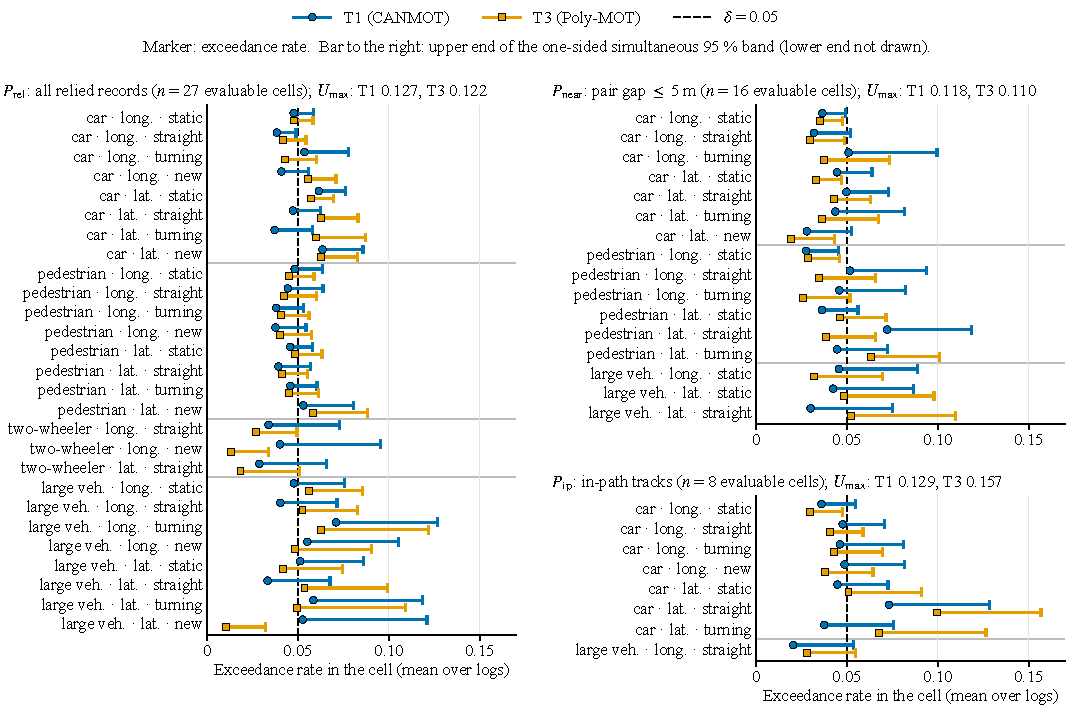
\includegraphics[width=\textwidth]{figs/fig02_mstar_cells.pdf}
\caption{M$^{*}$'s exceedance in every evaluable cell on Argoverse 2, run of record. Cells are object group $\times$ axis $\times$ course-change state, pooled over range, with records from at least 39 logs. Populations: $P_{\mathrm{rel}}$, all relied records; $P_{\mathrm{near}}$, pair gap $\leq$ 5 m; $P_{\mathrm{ip}}$, in-path tracks. Each marker is the cell's exceedance rate, the mean over logs of each log's share of exceeded records (T1, CANMOT: circles; T3, Poly-MOT: squares). Each bar runs to the upper end of the one-sided simultaneous 95~\% sup-t band from the log bootstrap over the population's evaluable cells. The band's lower end decides the flags and is not drawn; the dashed line is $\delta = 0.05$, and $U_{\max}$ is the largest upper end. In a simulation at Argoverse 2's cell sizes these simultaneous bounds covered only 38--55~\% of the time (Section V-E(c)), so they understate how large a cell exceedance the data allow.}
\label{fig:2}
\end{figure*}

\textbf{6. Operability against the informative comparators} (Table 4, Fig.~3).

\begin{figure}[!t]
\centering
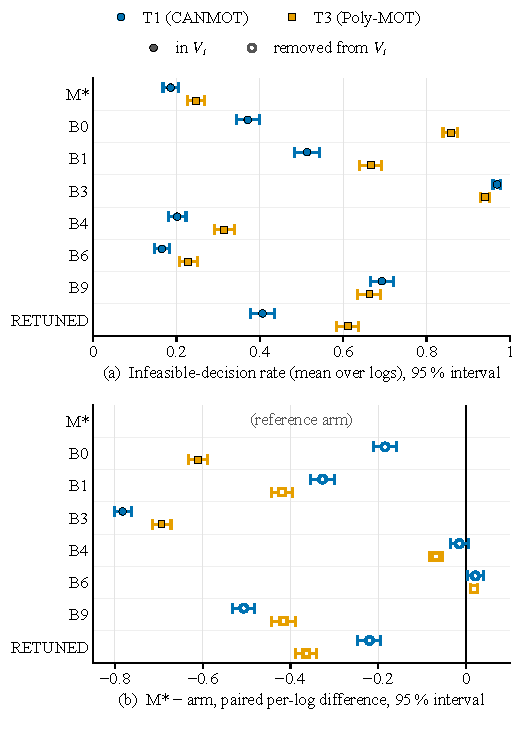
\includegraphics[width=\columnwidth]{figs/fig03_infeasible_arms.pdf}
\caption{Infeasible-decision rate per arm on Argoverse 2, run of record (375 logs, decision mode), with arms in the order of Table 4, for T1 (CANMOT, circles) and T3 (Poly-MOT, squares). (a) The rate, the mean over logs of each log's share of infeasible decisions, with its two-sided 95~\% log-bootstrap interval. (b) The paired per-log difference M$^{*}$ $-$ arm with its two-sided 95~\% percentile log-bootstrap interval, resampling whole logs. Filled markers in (b) are comparators that stayed in the comparison set $V_t$; open markers are comparators removed from $V_t$, which were flagged in one of their conditions at one-sided 0.99861. H1 compared M$^{*}$ with the members of $V_t$ at one-sided $1 - 0.0125/|V_t|$, not at the 95~\% level shown.}
\label{fig:3}
\end{figure}

\begin{itemize}
\item \textbf{B6} (M$^{*}$ without course-change strata) was shown above $\delta$ in five $P_{\mathrm{rel}}$ cells on each tracker and left $V_{t}$. Yet M$^{*}$ was \textbf{more} often infeasible than B6, by +0.021 [0.003, 0.039] on T1 and +0.018 [0.009, 0.027] on T3 (two-sided 95~\%): the course-change strata bought calibration in course-change cells (by design, Section V-D3) at a cost of about 0.02 in infeasibility (once tuned to pass, B6 needs more back-off than M$^{*}$: Sections V-E(a) and VI-A).
\item \textbf{B4} (one pooled conformal threshold) was shown above $\delta$ in 9 (T1) and 6 (T3) $P_{\mathrm{rel}}$ cells; M$^{*}$ $-$ B4 $= -0.016$ on T1 (upper bound at H2's Holm level, one-sided 0.995: 0.011) and $-$0.069 on T3 ($-$0.049). H2 confirms only that M$^{*}$'s price against B4 is below 0.03, not that M$^{*}$ is better.
\item \textbf{Matched validity,} how often a comparator family backs off once tuned to pass a screen, was beyond Form B. Its one piece pre-specified as descriptive, B0 rescaled on the training folds until it passes (RETUNED-HK1), found no qualifying scale in any fold on either tracker; the most conservative scale, $\times8$, was then used, as the plan specified, and was infeasible in 0.781 (T1) and 0.977 (T3) of decisions. Section V-E(a) extends this to every family and to a neutral screen.
\end{itemize}

\begin{table*}[!t]
\centering
\caption{Per arm and tracker on Argoverse 2 (decision mode; $P_{\mathrm{rel}}$ cells flagged at one-sided 0.95 for M$^{*}$, 0.99861 for comparators; V2 with its per-track reference; mean margins on each arm's own relied pairs, not comparable across arms; the last four columns are read from the CSVs of record and reported after review (amendment A3): progress ratio, mean executed back-off level $\lambda$, V2$_{\mathrm{exec}}$ (some relied constraint exceeded at the executed margin) and the share of decisions whose smallest enforced gap is below 1 m).}
\label{tab:4}
\scriptsize
\setlength{\tabcolsep}{2pt}
\renewcommand{\arraystretch}{1.15}
\begin{tabular}{@{}L{0.061\textwidth}L{0.084\textwidth}L{0.053\textwidth}L{0.039\textwidth}L{0.046\textwidth}L{0.039\textwidth}L{0.061\textwidth}L{0.084\textwidth}L{0.090\textwidth}L{0.039\textwidth}L{0.088\textwidth}L{0.069\textwidth}L{0.039\textwidth}L{0.039\textwidth}L{0.051\textwidth}@{}}
\hline
Tracker & Arm & Screen & $P_{\mathrm{rel}}$ & $P_{\mathrm{near}}$ & $P_{\mathrm{ip}}$ & Flagged & Infeasible & V2 (ref.) & V2$_{\mathrm{viol}}$ & Margin lat / long (m) & Progress & Mean $\lambda$ & V2$_{\mathrm{exec}}$ & Min gap $< 1$ m \\
\hline
T1 & M$^{*}$ & met & 0.044 & 0.038 & 0.040 & 0 / 27 & 0.186 & 0.491 (0.441) & 0.016 & 0.57 / 1.22 & 0.972 & 0.897 & 0.551 & 0.296 \\
T1 & B0 & -- & 0.034 & 0.026 & 0.050 & 3 / 26 & 0.371 & 0.395 (0.440) & 0.022 & 1.47 / 2.32 & 0.961 & 0.795 & 0.515 & 0.270 \\
T1 & B1 & -- & 0.013 & 0.016 & 0.030 & 1 / 26 & 0.513 & 0.188 (0.436) & 0.019 & 3.13 / 4.34 & 0.957 & 0.700 & 0.375 & 0.272 \\
T1 & B3 & in $V_{t}$ & 0.002 & 0.005 & 0.001 & 0 / 24 & 0.969 & 0.033 (0.411) & 0.007 & 10.49 / 12.29 & 0.974 & 0.128 & 0.745 & 0.321 \\
T1 & B4 & -- & 0.054 & 0.038 & 0.077 & 9 / 27 & 0.202 & 0.520 (0.441) & 0.026 & 1.02 / 1.60 & 0.972 & 0.888 & 0.578 & 0.288 \\
T1 & B6 & -- & 0.047 & 0.041 & 0.047 & 5 / 27 & 0.165 & 0.501 (0.441) & 0.023 & 0.54 / 1.73 & 0.971 & 0.911 & 0.548 & 0.287 \\
T1 & B9 & -- & 0.012 & 0.005 & 0.020 & 1 / 25 & 0.693 & 0.158 (0.434) & 0.014 & 3.59 / 3.59 & 0.955 & 0.505 & 0.527 & 0.268 \\
T1 & RETUNED & -- & 0.029 & 0.023 & 0.047 & 2 / 26 & 0.407 & 0.361 (0.440) & 0.022 & -- & 0.960 & 0.771 & 0.501 & 0.270 \\
T3 & M$^{*}$ & met & 0.043 & 0.032 & 0.040 & 0 / 27 & 0.247 & 0.496 (0.441) & 0.018 & 0.65 / 1.93 & 0.973 & 0.858 & 0.580 & 0.297 \\
T3 & B0 & in $V_{t}$ & 0.004 & 0.003 & 0.003 & 0 / 25 & 0.858 & 0.072 (0.431) & 0.013 & 5.44 / 6.66 & 0.965 & 0.302 & 0.604 & 0.292 \\
T3 & B1 & -- & 0.016 & 0.010 & 0.021 & 0 / 25 & 0.666 & 0.228 (0.433) & 0.024 & 2.95 / 3.58 & 0.968 & 0.495 & 0.575 & 0.284 \\
T3 & B3 & in $V_{t}$ & 0.001 & 0.001 & 0.000 & 0 / 24 & 0.941 & 0.030 (0.409) & 0.009 & 8.83 / 10.57 & 0.972 & 0.182 & 0.678 & 0.308 \\
T3 & B4 & -- & 0.061 & 0.044 & 0.112 & 6 / 26 & 0.315 & 0.572 (0.441) & 0.049 & 1.07 / 1.39 & 0.969 & 0.802 & 0.643 & 0.288 \\
T3 & B6 & -- & 0.049 & 0.036 & 0.044 & 5 / 27 & 0.229 & 0.529 (0.441) & 0.023 & 0.63 / 2.08 & 0.973 & 0.866 & 0.597 & 0.295 \\
T3 & B9 & -- & 0.014 & 0.005 & 0.016 & 1 / 26 & 0.663 & 0.177 (0.435) & 0.018 & 3.29 / 3.29 & 0.959 & 0.534 & 0.523 & 0.269 \\
T3 & RETUNED & -- & 0.026 & 0.014 & 0.045 & 2 / 25 & 0.611 & 0.316 (0.438) & 0.028 & -- & 0.960 & 0.580 & 0.568 & 0.278 \\
\hline
\end{tabular}
\end{table*}

An arm with no flagged $P_{\mathrm{rel}}$ cell can still be shown above $\delta$, through $P_{\mathrm{near}}, P_{\mathrm{ip}}$, a family cell or a pooled cell; each comparator's conditions are in Supplement S4.

\textbf{7. The trade-off.} M$^{*}$ buys feasibility with more exceeded constraints per decision. Its V2 (decisions with some relied constraint exceeded) is 0.491 (T1) and 0.496 (T3), about 0.05 above the per-track reference $1 - 0.95^{n_{\mathrm{tracks}}}$ as on development (a yardstick, not a null: it assumes one independent constraint per track, whereas V2 spans four check times per track), and up from B0's 0.395 (T1) and 0.072 (T3). Its V2$_{\mathrm{viol}}$ (decisions with a violation at the chosen plan) falls on T1 $(0.022 \to 0.016)$ and rises on T3 $(0.013 \to 0.018)$ relative to B0. Section V-E(f) shows the infeasibility--violation trade-off for every arm and what infeasible decisions do.

\textbf{8. Secondary claims} (Table 5). \textbf{H2 is confirmed:} a bound on a price, not superiority. \textbf{H4 is not confirmed: M$^{*}$'s nuScenes-fitted thresholds did not carry over.} With every arm fitted on nuScenes, M$^{*}$ is shown above $\delta$ on both trackers, in longitudinal cells and in the in-path pooled cell (pooled $P_{\mathrm{ip}}$ exceedance 0.070, HK1c bound 0.089); Holm's sequence stopped at H6b, and H4 also fails its own level. The procedure re-fitted on new data passed (H1); how many Argoverse 2 logs a re-fit needs is in Section V-E(g). \textbf{H8 holds} only as a partial replication (Section V-B). The other claims, H3, H6a, H6b, H9, H10, Form A and H7 (the method-stage rule on the in-path audit items, fitted on nuScenes), are reported in full in Supplement S4.1.

\begin{table*}[!t]
\centering
\caption{Claim statuses (family S by Holm at 0.025, gated on H1, $p = (k + 1)/(B + 1)$; H6a and H7 no-flag statements; H8 family P at its own 0.025; H9, H1-P, H5 and Form A descriptive; details in Supplement S4).}
\label{tab:5}
\footnotesize
\setlength{\tabcolsep}{4pt}
\renewcommand{\arraystretch}{1.15}
\begin{tabular}{@{}L{0.050\textwidth}L{0.443\textwidth}L{0.107\textwidth}L{0.347\textwidth}@{}}
\hline
Claim & What it tests & $p$ (Holm level) & Status \\
\hline
H1 & Form B on T1 and T3 (primary) & -- & holds \\
H2 & M$^{*}$'s price against B4 is $\leq 0.03$ in infeasible-decision rate & $2.5 \times 10^{-5}$ (0.005) & confirmed \\
H6b & method stage: B4 flagged where the method-stage rule is not, with a positive paired difference & 0.0199 (0.00625) & not confirmed \\
H10 & M$^{*}$ against B6: B6's flags, and M$^{*}$ $-$ B6 $\leq 0.03$ & 0.172 (0.00833) & not confirmed \\
H3 & the trajectory-level M$^{*}$Jx & 1.000 (0.0125) & not confirmed \\
H4 & H1 with every arm fitted on nuScenes & 1.000 (0.025) & not confirmed \\
H6a & the method-stage rule on the in-path audit items, fitted within Argoverse 2, flagged nowhere & -- & holds \\
H7 & the method-stage rule on the in-path audit items, fitted on nuScenes, flagged nowhere & -- & does not hold \\
H8 & the diagnosis of Section V-B replicates (T1, B0, in-path cars, lateral, 2 s) & -- & holds (partially; Section V-B) \\
H9 & Trajectron++~\cite{Salzmann2020} with DP-SCRC on the in-path relied items & -- & no cell flagged; floor not met \\
H1-P & H1 on the 150 validation logs with the public LT3D detector & -- & $P_{\mathrm{near}}$ floor not met \\
H5 & H1 on the 150 validation logs with the public VoxelNeXt detector~\cite{Chen2023voxelnext} & -- & $P_{\mathrm{near}}$ floor not met \\
Form A & M$^{*}$ less often infeasible than B0, B1, B4 and B9 & -- & not met on T1 (one-sided 0.99375 upper bound +0.010 against B4); met on T3 \\
\hline
\end{tabular}
\end{table*}

\textbf{9. A third tracker, and the rest of the record.} On AB3DMOT, M$^{*}$, re-fitted within Argoverse 2 for this tracker too, does not pass the screen: pooled $P_{\mathrm{rel}}$ exceedance 0.061 (lower bound 0.057), infeasible in 0.891 of decisions. The GO therefore covers the two registered trackers only; Section V-E(h) diagnoses the failure. The three 150-log routes fail the $P_{\mathrm{near}}$ floor, loop mode was not run as registered (an exploratory replay is in Section V-E(i)), and the plan's optional question on the trajectory-level joint loss was not tested; Supplement S4 reports every pre-specified output.

\textbf{10. A separate re-derivation of the results.} A re-implementation within the project, not an independent one, re-derived the analysis from the registered plan without opening the analysis code's statistical functions: 108,059 comparisons agree and none disagrees, and H1 held in 20 of 20 alternative seed sets (Supplement S4).

\textbf{11. Deviations.} Three events were logged before the affected steps were repeated, and two transfer runs were started by hand with their frozen commands. No rule, input, seed or analysis changed (Supplement S5).

\subsection{Exploratory analyses added after the verdict}
\textbf{Status of these analyses.} They answer questions that internal reviews of earlier drafts raised and the registered test could not. They were specified after the verdict and after reading the registered outputs, in a plan whose hash we recorded ourselves (no third-party timestamp) and five amendments (A1--A5), each hash-locked before its own outputs were computed. They are exploratory, change no registered result and carry no family-wise error control across analyses. Every output the plan or an amendment specifies is reported here or in Supplement S6, whichever way it points; quantities specified by neither are marked \emph{(added)}. The frozen code is imported and run unchanged by a new runner, which first reproduced the runs of record exactly (decisions, back-off levels and per-cell counts); at $B = 4000$ its screen gives the record's status for 98 of 99 arms, the exception (sweep point B0a4 on T1) having its deciding bound 0.9 Monte Carlo standard errors from its threshold.

\textbf{(a) Back-off at matched screen status.} Each comparator family is tuned until it passes a screen, then compared with M$^{*}$ there: B0 by scale (or nominal level), B4, B6 and B9 by nominal level $\delta'$, refitted by their own rule, on a grid that ends at 0.005 (smaller levels need more calibration logs than a training split has; Supplement S6.2). Each held-out fold uses the least conservative point that passes on the other four folds; a family with no passing point in some fold has \textbf{no matched point}, and its in-sample best is reported, with no conservative substitute (Table 6). The screens are \textbf{the registered screen,} whose cells are M$^{*}$'s own strata (Section V-D3); \textbf{a neutral screen} (amendment A4): no flagged cell in $P_{\mathrm{rel}}, P_{\mathrm{near}}$ or $P_{\mathrm{ip}}$ on the seven partitions of (b), plus HK1c on each population, with M$^{*}$'s own level $\delta'$ tuned on the same grid; and \textbf{a reduced neutral screen} (amendment A5), the same without track speed (P1) and track age (P3), coarse functions of the variables that define M$^{*}$'s ``static'' and ``new'' course-change states.

\begin{table*}[!t]
\centering
\caption{Back-off at matched screen status (cross-fitted; level $\to$ infeasible-decision rate; paired M$^{*}$ $-$ composite infeasible rate with 95~\% log-bootstrap interval, conditional on the selected levels (the selection is not re-run in the bootstrap); V2$_{\mathrm{exec}}$ on the reduced screen. \dag{} B9 still passes at the least conservative grid point $(\delta' = 0.05)$ in two to five of the five folds, so its matched point is censored by the grid and its contrast is not a matched comparison. The registered-screen results are in Supplement S6.2).}
\label{tab:6}
\footnotesize
\setlength{\tabcolsep}{3pt}
\renewcommand{\arraystretch}{1.15}
\begin{tabular}{@{}L{0.060\textwidth}L{0.184\textwidth}L{0.155\textwidth}L{0.155\textwidth}L{0.147\textwidth}L{0.155\textwidth}L{0.067\textwidth}@{}}
\hline
Tracker & Family & Neutral screen (P1--P7): level $\to$ infeasible & M$^{*}$(0.03) $-$ composite & Reduced screen (P2, P4--P7): level $\to$ infeasible & M$^{*}$(0.03) $-$ composite & V2$_{\mathrm{exec}}$ (reduced) \\
\hline
T1 & M$^{*}$ & $0.03 \to 0.260$ & -- & $0.03 \to 0.260$ & -- & 0.448 \\
T1 & B6 (no course-change strata) & $0.02 \to 0.493$ & $-$0.232 [$-$0.258, $-$0.207] & $0.03\text{--}0.04 \to 0.298$ & $-$0.038 [$-$0.063, $-$0.012] & 0.475 \\
T1 & B0 (scale or level) & $\times2\text{--}3$ or $0.005 \to 0.562$ & $-$0.302 [$-$0.330, $-$0.275] & $0.02 \to 0.468$ & $-$0.208 [$-$0.234, $-$0.181] & 0.476 \\
T1 & B4 (one pooled threshold) & $0.015\text{--}0.02 \to 0.533$ & $-$0.272 [$-$0.299, $-$0.246] & $0.02\text{--}0.03 \to 0.447$ & $-$0.187 [$-$0.214, $-$0.160] & 0.448 \\
T1 & B9 (norm ball), censored\dag{} & $0.04\text{--}0.05 \to 0.700$ & $-$0.439 [$-$0.465, $-$0.415] & $0.05 \to 0.693$ & $-$0.432 [$-$0.458, $-$0.406] & 0.527 \\
T3 & M$^{*}$ & $0.03 \to 0.351$ & -- & $0.03 \to 0.351$ & -- & 0.504 \\
T3 & B6 & $0.02 \to 0.430$ & $-$0.079 [$-$0.092, $-$0.067] & $0.02\text{--}0.03 \to 0.383$ & $-$0.033 [$-$0.045, $-$0.021] & 0.465 \\
T3 & B0 & $\times0.333 \to 0.732$ & $-$0.382 [$-$0.406, $-$0.360] & $\times0.25\text{--}0.333 \to 0.708$ & $-$0.357 [$-$0.380, $-$0.334] & 0.559 \\
T3 & B4 & $0.01\text{--}0.015 \to 0.701$ & $-$0.350 [$-$0.374, $-$0.328] & $0.015 \to 0.633$ & $-$0.283 [$-$0.303, $-$0.262] & 0.516 \\
T3 & B9, censored\dag{} & $0.04\text{--}0.05 \to 0.692$ & $-$0.341 [$-$0.371, $-$0.313] & $0.05 \to 0.663$ & $-$0.312 [$-$0.341, $-$0.284] & 0.523 \\
\hline
\end{tabular}
\end{table*}

\begin{itemize}
\item \textbf{On the registered screen only B6 on T3 has a matched point} (0.015, infeasible in 0.486 of decisions against M$^{*}$'s 0.247; M$^{*}$ $-$ B6 $-$0.240 [$-$0.256, $-$0.224]); B0, B4 and B9 have none on either tracker, and B6 on T1 lacks one in one fold. For B4 and B9 this is mostly not a flag: once conservative enough to have no flag, they keep too few relied records to meet the floor of power-qualified near-gap cells. The most conservative grid points that the exploratory plan substituted in such folds are not matched comparisons and are not used as such (in-sample bests and substitutes: Supplement S6.2).
\item \textbf{On both neutral screens M$^{*}$ does not pass at its registered level:} at $\delta' = 0.05$ it is flagged in the five cells of (b) (on T1, four low-quality-track cells and one slow-track cell), and on the reduced screen in those that remain. From $\delta' = 0.03$ it passes both in every fold, and the registered screen too; every comparator composite matched on either neutral screen is flagged on the registered screen.
\item \textbf{What sets the matched levels} (Supplement S6.22). M$^{*}$'s level is set on both neutral screens by detection score (P4, score 0.4--0.5), on T1's neutral screen together with a slow-track cell (P1, 0.5--3 m/s). The comparators' levels are set on the neutral screen mostly by track speed (P1, 3--8 m/s), a partition related to M$^{*}$'s strata, and on the reduced screen by detection score, ego speed, track length and lidar points (P4, P5, P2, P6). B9 passes at the least conservative grid point in every fold of the reduced screen and in four (T1) and two (T3) folds of the neutral screen; in T3's other three folds its level is set by track speed.
\item \textbf{M$^{*}$ at 0.03 backs off less often than every comparator family matched within the grid} (B0, B4 and B6), on both neutral screens, every interval below 0: by 0.23--0.30 (T1) and 0.08--0.38 (T3) on the neutral screen, and by 0.04--0.21 (T1) and 0.03--0.36 (T3) on the reduced one, where the advantage over B6 shrinks to 0.04 (T1) and 0.03 (T3). B9's composites back off 0.31--0.44 more often than M$^{*}$, but because B9 is censored by the grid these gaps overstate the gain at matched status.
\item \textbf{Exceedance at the executed margin is similar, except against B6 on T3.} On the reduced screen M$^{*}$'s V2$_{\mathrm{exec}}$ is 0.448 against 0.448--0.527 (T1) and 0.504 against 0.465--0.559 (T3; B6 has the 0.465, with overlapping marginal intervals: M$^{*}$ [0.480, 0.529], B6 [0.441, 0.490]; no paired interval was computed), and its V2$_{\mathrm{viol}}$ is the lowest of the five on both trackers (0.013 and 0.015). On the neutral screen M$^{*}$'s V2$_{\mathrm{exec}}$ is lower than, or within the interval of, each composite's except B6 on T3 (+0.054 [0.043, 0.066]): against the closest comparator, M$^{*}$'s smaller back-off comes with more exceedance at execution.
\item \textbf{Points that pass both the registered and the neutral screen} cost more again: for example B6 at 0.01 (T1, infeasible 0.678) and 0.015 (T3, 0.486), B4 at 0.01 (T1, 0.695), B9 at 0.02 (0.822 and 0.817) and B0 at $\times4$ (T1, 0.660) and $\times0.5$ (T3, 0.781), against M$^{*}$ at 0.03 (0.260 and 0.351). What the course-change strata buy is discussed in Section VI-A (registered-level comparison: Section V-D6).
\end{itemize}

\textbf{(b) Validity on partitions no method stratifies on directly.} Every arm is also screened, by the same flag rule, on seven partitions (Table 7): track speed, track length, track age, detection score, ego speed, annotation lidar points and city (4 bins, or 6 cities, $\times 2$ axes). Track speed and track age are coarse functions of M$^{*}$'s course-change variables ((a)). The bins are those of the exploratory plan (\S{}2(b)); we chose them from their physical meaning and, by our account, without first inspecting the distributions of the relied records. Each partition and population is a family at one-sided simultaneous 0.95, with no control across the 21 families per tracker.

\begin{table}[!t]
\centering
\caption{Flagged cells on the seven partitions ($P_{\mathrm{rel}}$; summed over the partitions; no M$^{*}$ cell is flagged in $P_{\mathrm{near}}$ or $P_{\mathrm{ip}}$).}
\label{tab:7}
\footnotesize
\setlength{\tabcolsep}{3pt}
\renewcommand{\arraystretch}{1.15}
\begin{tabular}{@{}L{0.173\columnwidth}L{0.064\columnwidth}L{0.064\columnwidth}L{0.064\columnwidth}L{0.064\columnwidth}L{0.064\columnwidth}L{0.064\columnwidth}L{0.064\columnwidth}L{0.175\columnwidth}@{}}
\hline
Tracker & M$^{*}$ & B0 & B1 & B3 & B4 & B6 & B9 & matched arms of (a) and B8 \\
\hline
T1 & 5 & 7 & 1 & 0 & 22 & 13 & 0 & 0 \\
T3 & 5 & 0 & 1 & 0 & 24 & 14 & 1 & 0 (B8: 1) \\
\hline
\end{tabular}
\end{table}

\textbf{M$^{*}$ does not pass on every partition, and its failures share a pattern:} its flagged cells concentrate in low-quality tracks, and 7 of the 10 are lateral:

\begin{itemize}
\item detection score 0.4--0.5: T1 lateral 0.093 (simultaneous upper bound 0.109) and longitudinal 0.087; T3 lateral 0.088 (0.101) and longitudinal;
\item tracks one or two keyframes old: 0.065 (T1), 0.067 (T3);
\item annotations with 1--10 lidar points: 0.071 (T1), 0.076 (T3), and on T3 also 11--50 points;
\item one slow-track cell on T1: 0.5--3 m/s, longitudinal, 0.082.
\end{itemize}

On T3 M$^{*}$ is also flagged in two lateral distance cells of $P_{\mathrm{rel}}$, 20--40 m and $\geq 40$ m (lower bounds 0.051 and 0.050), although it stratifies on distance: where its strata fall back to coarser thresholds, ranges are pooled, and the scored relied records differ from the calibration items (Section IV-G). Corrected across the seven partitions (one-sided $1 - 0.05/7$; amendment A3), M$^{*}$ keeps 4 flags on T1 and 3 on T3; with lower bounds of 0.050--0.074 at the uncorrected level on both trackers (T3's 11--50-point lateral cell the lowest), the low-quality-track finding is credible, though still exploratory, without family-wise control. B4 and B6 at their registered levels are flagged far more often (22--24 and 13--14 cells), the matched conservative arms of (a) and B8 in none but one long-track cell (B8, T3). A track-quality stratum (score or track age) is the obvious extension, not fitted because it would be chosen after seeing these data.

\textbf{(c) How much the screen depends on its intervals.} Every decisive quantity of the registered screen was recomputed with a studentized log bootstrap and with a design-effect Wilson interval, and each method was simulated at Argoverse 2's cell sizes (Supplement S6.4; the two new methods and M$^{*}$'s own flag rate are \emph{(added)}). The record's flags are close to their level: with every cell at $\delta$, M$^{*}$ is flagged in a given population in 3--6~\% of data sets and in some population in 11~\% (T1) and 13~\% (T3), and a comparator truly at $\delta$ leaves $V_{t}$ in at most 0.3~\%. Its cell upper bounds are weaker than their label: as a simultaneous set they cover 38--55~\% of the time (26--52~\% at M$^{*}$'s observed cell rates), so $U_{\max}$ (Section V-D5) understates the cell exceedances the data allow. With the studentized bounds no status changes, but single cells up to M$^{*}$'s largest cell bound, 0.189 (in-path cars on T3), cannot be excluded. The Wilson interval flags a population at $\delta$ in 18--33~\% of data sets, so its flags carry little evidence.

\textbf{(d) M$^{*}$ at a reference that uses nothing after the decision time.} Refitted at two references that use no information after the decision time except the route, \textbf{(d1)} the planner's own plan at margin 0 and \textbf{(d2)} constant current speed along the route, M$^{*}$ keeps 98.7--99.8~\% of relied items on the same axis and side, its thresholds change by a median ratio of 1.000, it passes the screen on both trackers, and its infeasible rate changes by at most 0.0006. Under the leash, however, the margin-0 plan coincides with the logged progression in 96~\% of decisions: within log replay the hindsight reference does not drive M$^{*}$'s result, and closed loop is not tested by this check.

\textbf{(e) The obvious alternatives} (Table 8), each fitted by its own rule, cross-fitted on the same folds and items and run like M$^{*}$: \textbf{B5,} per-axis scalars; \textbf{B7,} a learned heteroscedastic scale (speed and turn rate) with one conformal threshold; \textbf{B8,} stratified variance matching, with M$^{*}$'s strata and the Gaussian quantile of the matched variance; and \textbf{Q-refit,} a process noise re-fitted for the 2 s horizon, one factor per class group, whose pre-specified grid's floor bound, so amendment A2, locked before any run, extended the grid down to no process noise.

\begin{table*}[!t]
\centering
\caption{Alternatives (registered screen; infeasible-decision rate; M$^{*}$ $-$ arm, paired, 95~\% interval).}
\label{tab:8}
\footnotesize
\setlength{\tabcolsep}{4pt}
\renewcommand{\arraystretch}{1.15}
\begin{tabular}{@{}L{0.233\textwidth}L{0.083\textwidth}L{0.079\textwidth}L{0.170\textwidth}L{0.083\textwidth}L{0.079\textwidth}L{0.170\textwidth}@{}}
\hline
Arm & T1 screen & T1 infeasible & T1 M$^{*}$ $-$ arm & T3 screen & T3 infeasible & T3 M$^{*}$ $-$ arm \\
\hline
M$^{*}$ & passes & 0.186 & -- & passes & 0.247 & -- \\
B5 per-axis scalars & shown above & 0.167 & +0.020 [0.001, 0.038] & shown above & 0.240 & +0.007 [$-$0.002, +0.017] \\
B7 learned scale & shown above & 0.154 & +0.033 [0.018, 0.047] & shown above & 0.263 & $-$0.017 [$-$0.030, $-$0.004] \\
B8 stratified variance matching & passes & 0.282 & $-$0.096 [$-$0.109, $-$0.084] & passes & 0.507 & $-$0.261 [$-$0.282, $-$0.240] \\
Q-refit (plan grid) & shown above & 0.271 & $-$0.085 [$-$0.108, $-$0.060] & floor only & 0.814 & $-$0.567 [$-$0.590, $-$0.544] \\
Q-refit (extended grid) & shown above & 0.230 & $-$0.044 [$-$0.067, $-$0.020] & floor only & 0.783 & $-$0.537 [$-$0.560, $-$0.515] \\
\hline
\end{tabular}
\end{table*}

\begin{itemize}
\item \textbf{The simpler fixes do not pass:} the two alternatives less often infeasible than M$^{*}$ on T1, per-axis scalars and a learned scale, are shown above $\delta$.
\item \textbf{B8 passes and is more conservative:} infeasible 0.10 (T1) and 0.26 (T3) more often than M$^{*}$, it leaves fewer constraints exceeded at its executed margin (V2$_{\mathrm{exec}}$ 0.354 and 0.438, against M$^{*}$'s 0.551 and 0.580). It has M$^{*}$'s strata but sets each margin from the matched variance instead of the one-sided tail.
\item \textbf{Re-fitting the process noise does not pass.} The fit asks for \emph{less} process noise over 2 s for most class groups (T1's pedestrians get factors 1--4), and the extended grid is again at its floor, $q = 0$, on T3 and for T1's cars. On T1 the arm is shown above $\delta$ (in-path pooled exceedance 0.070 and 0.080); on T3 even $q = 0$ leaves the covariance too wide, because the tracker's posterior part already is, so the arm fails a floor and is infeasible in about 0.8 of decisions. One global scale of the raw covariance (RETUNED) is also shown above $\delta$ on both trackers (Table 4).
\end{itemize}

\textbf{(f) What an infeasible decision costs.} At an infeasible decision ($\lambda < 1$, Section V-A) the planner cannot keep its per-constraint risk statement (Proposition 1 covers feasible decisions only) and takes the candidate with the largest progress at the reduced margin; the emergency stop depends on margin 0 only and is the same for every arm (0.004 of decisions on T1, 0.002 on T3, 0.006 on AB3DMOT). Amendment A3 asked what the back-off costs (Table 4; Supplement S6.13):

\begin{itemize}
\item \textbf{Progress in decision mode.} Each decision restarts from the logged state, so decision-mode progress measures only the one-step cost of a back-off. It is small: every arm of record is within 0.02 of M$^{*}$'s progress ratio, A3's pre-fixed threshold for no cost, except six of the most conservative B0 sweep points on T1, RETUNED-HK1 among them (0.020--0.023 less), and the zero-margin arm Z0 (0.022--0.023 more on both trackers). B3, for example, executes $\lambda = 0$ in most decisions on T1 and still matches M$^{*}$'s one-step progress. At the neutral-screen matched points the differences are resolved but below that threshold: M$^{*}$ makes 0.010--0.014 more on T1 and 0.004--0.009 more on T3, every interval above 0.
\item \textbf{Progress in loop mode} (descriptive; (i) and Supplement S6.18). The replayed arms are M$^{*}$, B0, B4 and B6 at their registered levels (M$^{*}$ at $\delta = 0.05$), B8, and the exploratory plan's B6 composite; none is at a neutral-matched point, and their progress differences do not follow back-off frequency: on T1, B6 backs off less often than M$^{*}$ (infeasible frames $-$0.037 [$-$0.052, $-$0.021] relative to M$^{*}$) yet makes 0.027 [0.013, 0.040] less progress, and B4 backs off about as often yet makes 0.052 [0.036, 0.068] less. As amendment A4 fixed, this replay ranks nothing.
\item \textbf{The designed margin.} M$^{*}$ keeps it in 81~\% (T1) and 75~\% (T3) of decisions.
\item \textbf{Exceedance at the executed margin.} At the registered level, the conservative arms that pass leave fewer relied constraints exceeded at the margin they execute: V2$_{\mathrm{exec}}$ is 0.354 for B8 and 0.469 for RETUNED-HK1 on T1, against M$^{*}$'s 0.551, and 0.438 for B8 on T3, against 0.580. Arms that back off to near-zero margins leave more (B3: 0.745 on T1). At matched screen status ((a)), the difference largely disappears.
\item \textbf{Close approaches.} The share of decisions whose smallest enforced gap is below 1 m is 0.27--0.32 for every arm of Table 4; M$^{*}$'s is 0.296 (T1) and 0.297 (T3).
\item \textbf{Selection in the screen.} The screen scores each arm's relied records at its full margin, and the pairs a backed-off decision leaves unsatisfied at full margin drop out (Appendix B), so a conservative arm is screened on fewer records (Section IV-A), and its low exceedance partly reflects that selection.
\end{itemize}

\textbf{Reading.} M$^{*}$'s lower infeasible rate means that the planner keeps the margin rule it was designed with more often. In decision mode this comes with one-step progress differences below A3's no-cost threshold; the closed-loop replay is descriptive and ranks nothing. We do not claim that M$^{*}$ makes the planner safer or more efficient.

\textbf{Fig.~4} shows the arms of record, the B0 sweep, the matched composites of (a) (B9's marked as censored) and B8 as infeasible rate against V2, V2$_{\mathrm{exec}}$ and V2$_{\mathrm{viol}}$. \emph{(added)} At M$^{*}$'s V2 of about 0.49, scaling the raw covariance is infeasible in about 0.28 of decisions on T1 (M$^{*}$: 0.186) and 0.44 on T3 (0.247), by linear interpolation of the sweep. No arm of record is at or below M$^{*}$ on both infeasible rate and V2$_{\mathrm{viol}}$ on any tracker, and every other arm of record that passes the screen is infeasible in at least 0.66 of decisions; the exploratory B8 of (e) passes at 0.282 and 0.507.

\begin{figure*}[!t]
\centering
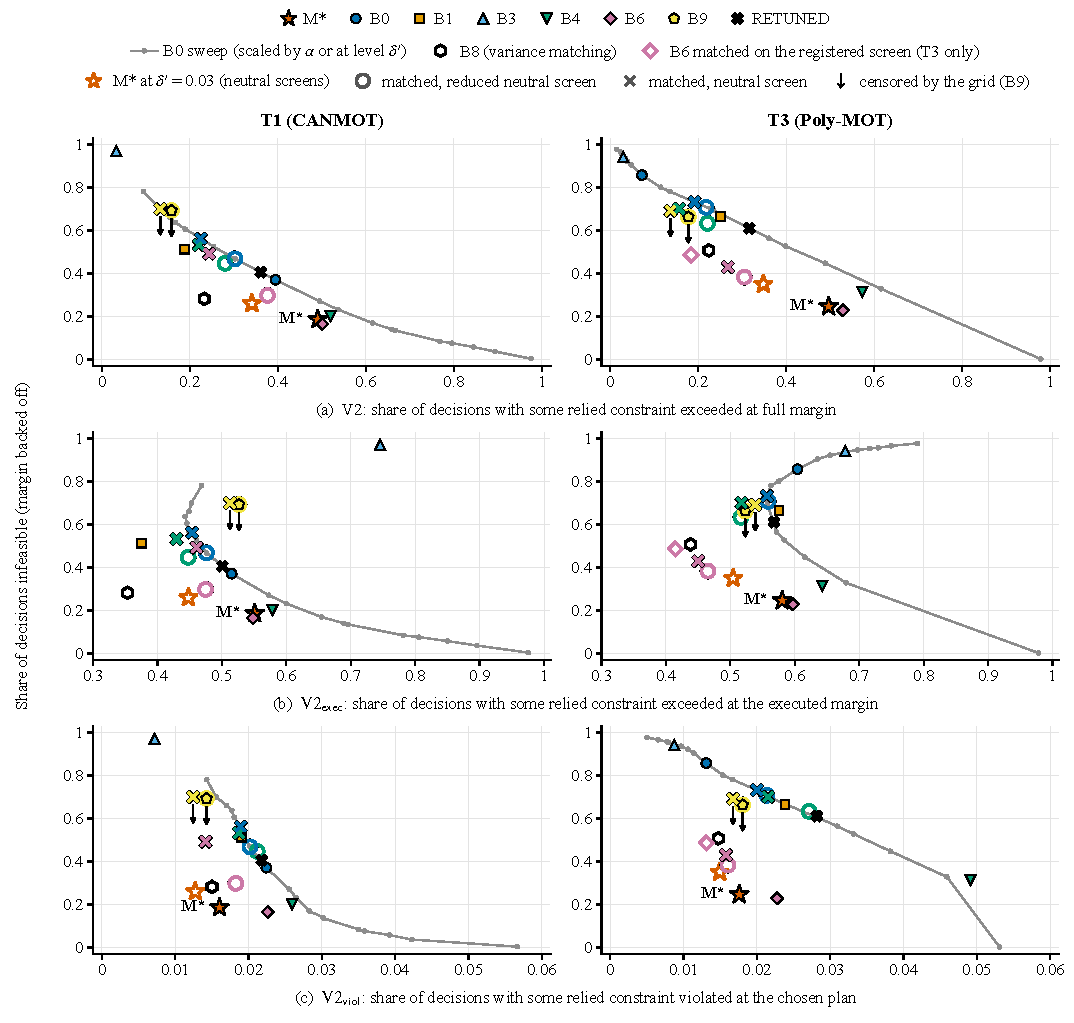
\includegraphics[width=\textwidth]{figs/fig04_tradeoff_v04.pdf}
\caption{Infeasible-decision rate, the share of decisions at which the planner backs off its margin, against three exceedance measures on Argoverse 2, for T1 (CANMOT) and T3 (Poly-MOT); log means over 375 logs, decision mode. (a) V2, the share of decisions with some relied constraint exceeded at full margin; (b) $\mathrm{V2}_{\mathrm{exec}}$, the same at the executed margin; (c) $\mathrm{V2}_{\mathrm{viol}}$, the share with some relied constraint violated at the chosen plan. Filled markers are the arms of record. The gray line joins the B0 sweep (raw covariance scaled by $\alpha$ or set at level $\delta'$) in order of V2, and its $\delta' = 0.5$ end coincides with the zero-margin arm Z0. The other markers are post-registration exploratory points, each composite picking every fold's level on the other four folds: B8; B6 matched on the registered screen, drawn for T3 only (on T1 one fold's level is substituted, so the composite is not a matched point); M$^{*}$ at $\delta' = 0.03$, matched on both neutral screens (hollow star); and, in each family's color, the B0, B4, B6 and B9 composites matched on the neutral screen (seven partitions no method stratifies on directly; crosses) and on the reduced neutral screen (without track speed and track age; rings). B9 passes at the least conservative grid point ($\delta' = 0.05$) in two to five of the five folds, so its matched point is censored by the grid (arrows); its rings sit on the B9 arm of record. Drawn offsets, so that no marker is hidden: the B9 crosses, about 4 pt, in T1 (a)--(c) and T3 (a) and (b); B8 in T1 (c), 7 pt to the right; B1 in T3 (a), about 5 pt to the right; and B6 matched on the registered screen in T3 (a)--(c), 5--6 pt to the left. Elsewhere, crosses are drawn above the markers of record and these above the rings, so touching markers stay visible. Z0, the learning-curve and alternative-reference refits and the other exploratory arms are not shown; every plotted value is listed in the supplementary table.}
\label{fig:4}
\end{figure*}

\textbf{(g) How many logs a re-fit needs} (Supplement S6.8). M$^{*}$ was refitted on $n$ of the 300 training logs per held-out fold, with 3 seeded repeats for $n < 300$. From 200 logs every repeat passes, at an infeasible rate within 0.02 of the full fit (0.005--0.017); at 50--100 logs most strata fall back to coarse thresholds, and on T1 single cells are still flagged in four of six repeats; at 25 logs most fits are impossible. On this indicative evidence (3 repeats, a low-power screen), a deployment should plan for roughly 200 annotated logs of about 15 s (50 minutes of driving) per tracker and domain for M$^{*}$ at $\delta = 0.05$ judged by the registered screen, and more at smaller levels (Section IV-C): the level that passes both neutral screens, $\delta' = 0.03$, needs at least 33 logs per own-threshold stratum and plausibly more logs overall.

\textbf{(h) Why AB3DMOT fails} (descriptive). Of the registered cells, only the pooled $P_{\mathrm{rel}}$ cell fails (Section V-D9). On the seven partitions of (b), M$^{*}$ on AB3DMOT is flagged in 16 $P_{\mathrm{rel}}$ cells (11 after the correction across partitions), spread over all seven, the low-score bin included. Unlike that of T1 and T3, AB3DMOT's planner population is dominated by weak and unmatched tracks (Table 9):

\begin{table}[!t]
\centering
\caption{What AB3DMOT's planner population is made of (descriptive; shares of relied records and of enforced pairs).}
\label{tab:9}
\footnotesize
\setlength{\tabcolsep}{3pt}
\renewcommand{\arraystretch}{1.15}
\begin{tabular}{@{}L{0.502\columnwidth}L{0.232\columnwidth}L{0.212\columnwidth}@{}}
\hline
 & AB3DMOT & T1 and T3 \\
\hline
relied records from tracks with detection score below 0.5 & 0.41 & 0.08 \\
enforced pairs whose track has no annotated object (false-positive tracks) & 0.40 (35.8 per decision) & 0.12 (6.9 per decision) \\
\hline
\end{tabular}
\end{table}

False-positive tracks are not the main cause of AB3DMOT's high infeasible rate: removing every unmatched track from the planner's input (amendment A4) lowers M$^{*}$'s infeasible rate only from 0.891 to 0.757, less than the halving that A4 fixed in advance as the threshold for a main driver, and M$^{*}$ is still flagged. The low-score share is reported as description; a score-aware stratum or a filter before calibration is the natural remedy, and was not tested.

\textbf{(i) Beyond the registered harness} (amendment A4). Enlarging the ego from nuScenes' $4.1 \times 1.8$ m to $4.9 \times 1.9$ m leaves M$^{*}$ passing the screen on both trackers (infeasible 0.208 on T1 and 0.270 on T3). \textbf{Loop mode} (descriptive; Supplement S6.18): each log was also replayed in closed loop with non-reactive agents (1,054 episodes per arm and tracker). At-fault collisions with tracked agents per 1,000 episodes were 29 for M$^{*}$, 46 for B0 and 48 for the B6 composite on T1, and 25, 38 and 39 on T3. Paired per episode, M$^{*}$ had fewer than B0 (T1 $-$0.017 [$-$0.033, $-$0.002]; T3 $-$0.013 [$-$0.027, $-$0.002]) and the B6 composite of the exploratory plan, which on T1 has one substituted fold ($-$0.019 [$-$0.035, $-$0.006]; $-$0.014 [$-$0.025, $-$0.005]); the other intervals include 0. The harness is far from a deployable planner, non-reactive agents bias loop-mode collisions in a direction we cannot sign, and an arm that backs off more often also drives differently: these numbers are descriptive and rank nothing.

\section{Discussion and Limitations}
\subsection{What the evidence supports}
\textbf{Registered, within one dataset.} A calibration fitted on the constraints a chance-constrained speed planner relies on was held near its level there, per stratum and pooled, on two trackers, in open-loop log replay. ``Held near its level'' means ``not shown above $\delta$'' at the stated power, with the pooled bounds of Table 3; never ``at most $\delta$'' in every cell~\cite{AltmanBland1995}. No equivalence claim is made~\cite{Schuirmann1987,Wellek2010}.

\textbf{Exploratory, added after the verdict.} On the relied constraints the raw covariance is mostly too wide, so M$^{*}$ mainly narrows it. Tuned to pass a screen on partitions that no method stratifies on directly, M$^{*}$ backs off its designed margin less often than every comparator family matched within the grid (B0, B4, B6), by 0.08--0.38 of decisions on seven partitions and by 0.03--0.36 without the two related to its strata (Section V-E(a)); B9's larger gap is censored by its grid.

\begin{itemize}
\item \textbf{The course-change strata.} At the registered level, B6 (M$^{*}$ without course-change strata) was less often infeasible than M$^{*}$ by 0.02, because it under-covers in course-change cells. Tuned to pass, it needs more back-off than M$^{*}$, but on the reduced screen only by 0.03--0.04, and on T3 it then leaves fewer constraints exceeded at execution (M$^{*}$ $-$ B6 +0.054 [0.043, 0.066] on the neutral screen). On this evidence the strata buy validity in course-change cells and little else; this is not a claim that they are necessary.
\item \textbf{What the lower back-off is worth.} The planner keeps the margin rule it was designed with more often. In the leashed decision-mode replay the one-step progress differences are below 0.02, A3's pre-fixed threshold for no cost; the closed-loop replay, with non-reactive agents and none of its arms at a neutral-matched point, ranks nothing (Section V-E(f), (i)). Neither replay supports a claim about safety or efficiency.
\end{itemize}

\textbf{Not supported:} that nuScenes thresholds can be reused on Argoverse 2 (H4 failed for M$^{*}$, and H7 for the method-stage rule on the in-path audit items); that the result extends to a third tracker (AB3DMOT failed the screen); or that M$^{*}$ passes on partitions it does not stratify (it under-covers low-quality tracks; Section V-E(b)). \textbf{Not tested at all:} anything per decision, any closed-loop property beyond the descriptive loop-mode replay of Section V-E(i), or safety.

\subsection{The proxy population and log replay}
M$^{*}$'s calibration items are defined at the logged ego trajectory (Section IV-A), a proxy for the constraints a deployed planner would create with its own plan, which depend on its margins; the logged human trajectory may avoid conflicts the planner would enter. The registered test's scoring of each arm on the relied constraints of its own chosen plan checks the proxy within decision mode without proving it, and refitting M$^{*}$ at two references that use nothing after the decision time changed its thresholds by a median ratio of 1.000, its validity not at all and its infeasible rate by at most 0.0006 (Section V-E(d)). Log replay still carries the logged trajectory (path, leash and decision states, for every arm alike), and the planner chooses only the speed. Open-loop scores at logged states can disagree with closed-loop behavior~\cite{Dauner2023,Karnchanachari2024}; the loop-mode replay added after the verdict uses non-reactive agents and ranks nothing (Section V-E(i)).

\subsection{Per constraint, per decision and the level $\delta$}
$\delta = 0.05$ is a calibration level per relied constraint, not a safety target. On Argoverse 2 about one decision in two keeps some exceeded relied constraint (V2 0.491 and 0.496), because a decision holds about 13 tracks. A trajectory-level calibration that brings this near 0.05 costs 0.31--0.39 in infeasibility on development (Section V-C) and was not confirmed on Argoverse 2 (H3). A planner that allocates risk across constraints by Boole's inequality needs much smaller per-constraint levels, and these need more data: at $\delta = 0.01$ an own threshold needs $\geq 99$ logs per stratum (Section IV-C), and smaller levels proportionally more. Per-constraint calibration at 0.05 keeps the margin rule the planner was designed with honest on average along each constraint; it does not make a decision safe.

\subsection{Registration, blinding and what was seen before the freeze}
\textbf{The blinding was procedural} (Section V-D1). Supplement S10 lists from the records every computation made on the 375 test logs before the freeze (18 entries), classed by the most each read of the annotations: detector AP, tracking metrics and planner-record counts on the 150 validation logs from 1 Nov; detector AP on the 225 held-out logs after training; and detection, tracking and the 2 s propagation on all 375 logs before the text lock, with the registered tracking metrics held back. By the records, no computation used an annotation position after a decision time, and no exceedance, margin, infeasibility, V2 or NEES on Argoverse 2 was computed or seen before the freeze. The records cannot show that no other analysis was run (the public annotation files were on the analysis computer, and tools outside the guarded entry points write no log line), nor whether the author saw any pre-freeze metric.

\textbf{The nuScenes stages are weaker:} their hashes are self-recorded; one pre-freeze check previewed the diagnosis study's decision; the validation split was examined before the first nuScenes study and used to tune T1's process noise; and reviews were within the project, with only one audit an independent re-implementation. The Argoverse 2 re-derivation (Section V-D10) was likewise written within the project, not by an independent team.

\subsection{Design defects and omissions of the registered plan}
Each was in the frozen plan or its code, and none changed after the run: an ambiguous HK1c calibration rule (mean or minimum over development cells), whose margin 0.03 is our own value, motivated by the 98.4th percentile of a Beta(15, 286) law; an H6b $p$-value of resolution 1/201 (200 refit replicates), which, foreseeably, could pass its Holm level only with no exceedance at all; loop mode listed among the descriptive outputs but not run as registered, because the frozen commands allow decision mode only (Section V-E(i) runs it as an exploratory addition); an H9 ``seed-robust'' label in the frozen code stricter than the plan's wording (both readings are reported); a comparator removal step that is a plain Bonferroni split over nine conditions, at $1 - 0.0125/9$ each, not a false-coverage-rate method; a comparison set, fixed on development, without B5, B7, a re-fitted process noise and the published filters' own implementations (Section V-E adds the first three as exploratory arms); screen cells that are M$^{*}$'s strata (Section V-D3), with the pairs a backed-off decision leaves unsatisfied at full margin dropped (Section V-E(f)); and nuScenes' ego footprint, smaller than Argoverse 2's vehicle, which changes no status (Section V-E(i)).

\subsection{Data, trackers and transfer}
\textbf{The data and the trackers.} Two datasets, with one detector architecture trained separately for each (on Argoverse 2 for 2 class-balanced epochs, set by a compute cap, against the public checkpoint's 20; Supplement S9.15); three tracker settings on nuScenes, sharing detections and association; on Argoverse 2, trackers at their nuScenes parameters, at 2 Hz, with thin two-wheeler cells. \textbf{The certificate's population} is matched true-positive tracks still observable at the horizon: false-positive tracks enter the planner's constraints but not the certificate, and on AB3DMOT removing them does not explain most of the failure (Section V-E(h)).

\textbf{Transfer.} M$^{*}$'s nuScenes-fitted thresholds did not transfer to Argoverse 2, mostly in longitudinal cells (H4, Section V-D); the frame rate and the different dynamics are candidate causes, which we did not diagnose. A deployment must re-fit M$^{*}$ on in-domain annotated logs (300 per fold here; with fewer, see Section V-E(g)). Under covariate shift, weighted conformal prediction~\cite{Tibshirani2019} or online threshold updates~\cite{GibbsCandes2021} are natural remedies; neither was tested here.

\subsection{Not claimed}
\textbf{For the diagnosis:} miscalibration of the tracker's current-time output; a uniform lateral failure; that only the decision projection reveals the problem; or that no scalar can fix it. \textbf{For M$^{*}$:} that its course-change strata are necessary (Section VI-A); that it is the tightest method; that it makes the planner safer or more efficient; or any guarantee for one deployed rule, per object, per decision, in fallback strata or in closed loop. \textbf{For Argoverse 2:} validity in non-evaluable cells, along the objects' true axes, or outside the four groups; transfer; or safety. Proposition 5 certifies only along the estimated box axes, which are often wrong for T1 boxes (Section V-B).

\section{Conclusion}
A chance-constrained planner with linearized constraints consumes one-sided tails of a tracker's covariance along its constraint normals, a property the standard NEES check does not test. On nuScenes, a constant-velocity tracker's 2 s covariance is mis-shaped for in-path cars, yet on the constraints a speed planner relies on it is mostly too wide. M$^{*}$ calibrates on those relied constraints, per stratum, and returns a covariance the planner uses unchanged.

\textbf{The registered claim.} In a registered test on Argoverse 2, in open-loop log replay with a speed-only planner, M$^{*}$ re-fitted there was not shown above 5~\% in any evaluable cell of the relied constraints, on two trackers. The registered comparison was uninformative, and single cells up to about 0.16 (0.19 by a post-registration interval) cannot be excluded.

\textbf{The exploratory evidence.} In analyses added after the verdict, with each method tuned to pass a screen on partitions no method stratifies on directly, M$^{*}$ kept the planner on its designed margin in 3--38 percentage points more decisions than every comparator family matched within the grid. Against M$^{*}$ without its course-change strata the gain was small, and on one tracker it came with more exceedance at execution.

\textbf{The failures.} M$^{*}$ under-covers low-score and newly started tracks, failed its screen on a third tracker, AB3DMOT, and its thresholds did not transfer between datasets. What the paper offers is therefore a procedure to be re-fitted per tracker and domain, on roughly 200 annotated logs (an indicative figure), with track quality as the next stratum to add.

\textbf{Not claimed:} anything per decision, about safety, or in closed loop. $\delta$ is a calibration level per relied constraint, and about half of all decisions keep some exceeded constraint.

Code, plans, hashes, run logs and result files are released at \url{https://github.com/anandakopalli7/mstar-planner-matched-calibration}.

\section*{Tools and author responsibility}
The author conceived the study, determined its direction and objectives, and made the scientific decisions. Under the author's instructions, Claude (Anthropic) assisted with literature searches, mathematical derivations and checks, programming, analysis, and manuscript preparation. The author takes responsibility for the work.

\appendices
\section{\break Proofs}
This appendix proves Theorem 1(b), Proposition 3, with the conformal-risk-control step and the log as the unit, and Proposition 4. Every other statement of Sections III and IV is proved in Supplement S8, which reproduces the previous full appendix under its earlier labels and gives a label map (Section A.4). A tag [C: id] points to the numeric check of a statement in the released file \path{A_proofs_checks_v01.json}. Each check is exact (closed form or rational arithmetic), a one-dimensional quadrature, or a seeded Monte Carlo run with the stated tolerance.

Throughout, $\Phi$ and $\varphi$ are the standard normal distribution and density functions, $\bar{\Phi} = 1 - \Phi$, and $z_{1-\delta} = \bar{\Phi}^{-1}(\delta)$, with $\delta \in (0, \tfrac{1}{2})$. The setting (M1)--(M3) is that of Section III-A.

\subsection*{A.1 Theorem 1(b): a whole-vector test passed exactly with a direction above $\delta$}
\textbf{Theorem 1(b).} As in Theorem 1, $e = X - \hat{m}$ has the stated law given $I_{k}$, the export is $\hat{V}$, and the risk along $a$ is $P(a^{\top}e/\sqrt{a^{\top}\hat{V}a} > z_{1-\delta})$; the level is $\delta = 0.01$ unless stated. A whole-vector $\chi^{2}$ test can be passed exactly while the risk along some direction exceeds $\delta$. Let $R^{2} \sim \chi_{2}^{2}$ and let $\theta$ be an angle with any law, independent of $R$; set $e = R(\cos \theta, \sin \theta)$ and export $\hat{V} = I_{2}$.

\emph{Proof.}

\begin{enumerate}
\item[1.] \textbf{$N$ is exactly $\chi_{2}^{2}$.} $N = e^{\top}e = R^{2}$, whose law does not involve $\theta$. Every test that uses only the law of $N$, such as the $\chi^{2}$ test with any acceptance region, the ANEES test or the $p_{v}$ statistic, behaves exactly as under a calibrated Gaussian. For example, $P(N > \chi_{2;0.95}^{2}) = e^{-\chi_{2;0.95}^{2}/2} = 0.0500$ exactly.
\item[2.] \textbf{The risk along a direction.} Let $a_{\varphi} = (\cos \varphi, \sin \varphi)$. With $\hat{V} = I_{2}, U_{\varphi} = a_{\varphi}^{\top}e = R \cos(\theta - \varphi)$. Since $P(R > r) = P(R^{2} > r^{2}) = e^{-r^{2}/2}$ for $r \geq 0$ and $z = z_{1-\delta} > 0$,

\begin{equation*}
P(U_\varphi > z \mid \theta) = h(\theta - \varphi), \qquad h(\psi) = \exp\bigl(-z^2/(2\cos^2\psi)\bigr)\cdot\mathbf{1}\{\cos\psi > 0\},
\end{equation*}

so the risk along $a_{\varphi}$ is $\mathrm{risk}(\varphi) = E[h(\theta - \varphi)]$.
\item[3.] \textbf{The direction average is exactly $\delta$.} By Fubini's theorem and periodicity,

\begin{equation*}
\frac{1}{2\pi}\int_0^{2\pi} \mathrm{risk}(\varphi)\,d\varphi = E\Bigl[\frac{1}{2\pi}\int_0^{2\pi} h(\theta - \varphi)\,d\varphi\Bigr] = \frac{1}{2\pi}\int_0^{2\pi} h(\psi)\,d\psi.
\end{equation*}

The right-hand side is the risk when $\theta$ is uniform. Then $e \sim N(0, I_{2})$ and $U_{\varphi} \sim N(0, 1)$, so it equals $\bar{\Phi}(z) = \delta$. Since $\mathrm{risk}(\varphi)$ is continuous in $\varphi$ (dominated convergence), $\max_{\varphi} \mathrm{risk}(\varphi) \geq \delta$, with equality iff $\mathrm{risk}(\varphi) = \delta$ for every $\varphi$. So for \textbf{every} angle law whose directional risk is not constant, some direction has risk above $\delta$, while every $N$-based test is passed exactly.
\item[4.] \textbf{The example.} Let $\theta = \theta_{0} + \pi B$, with $\theta_{0} \sim N(0, s^{2})$ and $B$ a fair bit independent of $\theta_{0}$. The symmetry $\theta \mapsto \theta + \pi$ gives $E[e] = 0$. For $\cos \psi \neq 0$ exactly one of $h(\psi)$ and $h(\psi + \pi)$ is non-zero, and $h(\psi) + h(\psi + \pi) = \exp(-z^{2}/(2\cos^{2}\psi))$; hence, along $a_{0} = (1, 0)$,

\begin{equation*}
\mathrm{risk}(0) = \tfrac{1}{2}\cdot E\bigl[\exp\bigl(-z^2/(2\cos^2\theta_0)\bigr)\bigr].
\end{equation*}

One-dimensional quadrature at $z = z_{0.99}$ gives 0.02682, 0.01808 and 0.01214 for $s = 0.3$, 0.6 and 1.0. As $s \to 0$ the risk tends to $\tfrac{1}{2}e^{-z^{2}/2} = 0.0334$, and as $s \to \infty$ it tends to 0.01.
\item[5.] \textbf{What the joint test misses.} $\mathrm{Var}(e_{1}) = E[R^{2}]E[\cos^{2}\theta_{0}] = 1 + e^{-2s^{2}}$, which is 1.835 at $s = 0.3$: the covariance is wrong along $a_{0}$. The one-dimensional NEES along $a_{0}$, whose mean is $\mathrm{Var}(e_{1})$, detects it; the two-dimensional test cannot. $\blacksquare$ [C: \texttt{T1b}; the Monte Carlo check also confirms $p_{v95} = 0.050$ and the three risks to within $5 \times 10^{-4}$]
\end{enumerate}

\emph{A published example of this kind}~\cite{Forsling2025}: for $\Sigma = [[8, 1], [1, 2]]$ and $P = \mathrm{diag}(8, 2), E[N] = \mathrm{tr}(P^{-1}\Sigma) = 2$, while the whitened covariance $P^{-1/2}\Sigma P^{-1/2} = [[1, \tfrac{1}{4}], [\tfrac{1}{4}, 1]]$ has eigenvalues 0.75 and 1.25. [C: \texttt{T1b\_forsling}]

\subsection*{A.2 Proposition 3: certification with the log as the unit}
This section states Proposition 3 with the unit the registered test used, the log, and proves it from first principles, with the conformal-risk-control step written out.

\textbf{Setting.}

\begin{itemize}
\item \textbf{Logs and items.} A log $Z$ is a random element of a measurable space. A fixed \emph{item map} turns $Z$ into a finite, possibly empty, multiset of items ($x$, $U$), with features $x$ and score $U \in \mathbb{R}$. In the registered Argoverse 2 test a log is one drive segment of about 15 s. Its items are M$^{*}$'s calibration items (Section IV-A): every enforced pair at every decision state and calibrated check time, one item per object axis that separates the pair at the reference pose. The features include the check time and the in-path flag, because M$^{*}$ is fitted separately for each (check time, in-path flag). A \emph{stratum} $g$ is therefore a (check time, in-path flag, level-0 stratum) triple, and a \emph{cell} $C$ a (check time, in-path flag, coarser cell) triple. Items within a log may be arbitrarily dependent: they share tracks, consecutive decision states and the ego trajectory.
\item \textbf{Membership and loss.} $n_{g}(Z)$ is the number of $Z$'s items in $g$, and $A_{g}(Z) = \mathbf{1}\{n_{g}(Z) \geq 1\}$. For $A_{g}(Z) = 1$ the \emph{log loss} is

\begin{equation*}
L_g(Z; c) = \frac{1}{n_g(Z)}\cdot\sum_{\text{items of } Z \text{ in } g} \mathbf{1}\{U > c\}, \qquad c \in \mathbb{R} \cup \{+\infty\}.
\end{equation*}
\item \textbf{Calibration and threshold.} Calibration logs $Z_{1}, \dots, Z_{m}$; $I_{g} = \{i : A_{g}(Z_{i}) = 1\}$; $N_{g} = |I_{g}|$; $\hat{R}_{g}(c) = (1/N_{g})\sum_{i\in I_{g}} L_{g}(Z_{i}; c)$;

\begin{equation*}
\hat{c}_g = \inf\Bigl\{c \in \mathbb{R} : \frac{N_g}{N_g + 1}\cdot\hat{R}_g(c) + \frac{1}{N_g + 1} \leq \delta\Bigr\}, \qquad \text{with } \inf\emptyset = +\infty.
\end{equation*}
\end{itemize}

\textbf{Assumptions.}

\begin{itemize}
\item \textbf{(L1) I.i.d. logs.} $Z_{1}, \dots, Z_{m}$ and $Z_{\mathrm{test}}$ are independent and identically distributed. This is the modeling assumption of the test. It treats logs recorded in the same city or on the same day as independent draws from the population of logs. It is not testable from the data.
\item \textbf{(L2) A fixed item map.} The item map, the stratum map and every ingredient of $U$ are fixed without using $Z_{1}, \dots, Z_{m}$ or $Z_{\mathrm{test}}$. The ingredients include the detector, the tracker's $Q$ and $R, \sigma_{a}$, the cut-points and the planner that defines enforced pairs. In the registered test the detector was not trained on the 375 logs and both trackers keep their nuScenes parameters (Section V-D). The item map may use anything inside the log, including the logged future ego pose; this matters for Section IV-G, not here. If an ingredient was fitted on the evaluation logs, only a transductive reading holds instead (S8-Remark 4).
\item \textbf{(L3) Positive membership.} $P(A_{g}(Z) = 1) > 0$.
\end{itemize}

\textbf{Properties of the log loss.} For each log with $A_{g}(Z) = 1, c \mapsto L_{g}(Z; c)$:

\begin{itemize}
\item (F1) is non-increasing, because each $\mathbf{1}\{U > c\}$ is;
\item (F2) is right-continuous, because $\mathbf{1}\{U > c\} \to \mathbf{1}\{U > c_{0}\}$ as $c \downarrow c_{0}$ (for $U > c_{0}$ eventually $c < U$; for $U \leq c_{0}$ the indicator is always 0), and a finite average preserves this;
\item (F3) takes values in [0, 1], so it is bounded by $B = 1$;
\item (F4) satisfies $L_{g}(Z; +\infty) = 0$, and $L_{g}(Z; c) = 0$ for $c \geq$ the log's largest $g$-score;
\item (F5) satisfies $L_{g}(Z; c) = 1$ for $c$ below the log's smallest $g$-score.
\end{itemize}

\textbf{Lemma A.1 (conformal risk control, in the form used).}~\cite[Thm.~1]{Angelopoulos2024} states: if $L_{1}, \dots, L_{n+1}$ are exchangeable random functions of $\lambda$ that are non-increasing and right-continuous, with $L_{i}(\lambda_{\max}) \leq \alpha$ and $\sup_{\lambda} L_{i}(\lambda) \leq B < \infty$ almost surely, then $\hat{\lambda} = \inf\{\lambda : (n/(n + 1))\hat{R}_{n}(\lambda) + B/(n + 1) \leq \alpha\}$, with $\hat{\lambda} = \lambda_{\max}$ if the set is empty, satisfies $E[L_{n+1}(\hat{\lambda})] \leq \alpha$. We use it with $\lambda = c, \lambda_{\max} = +\infty, B = 1$ and $\alpha = \delta$. For completeness, here is the proof in this setting.

Let $\alpha \in (0, 1)$. Let $\ell_{1}, \dots, \ell_{n+1}$ be random functions on $\mathbb{R} \cup \{+\infty\}$ with values in [0, 1] such that:

\begin{itemize}
\item (C1) $(\ell_{1}, \dots, \ell_{n+1})$ is exchangeable;
\item (C2) each $\ell_{i}$ is non-increasing;
\item (C3) each $\ell_{i}$ is right-continuous;
\item (C4) each $\ell_{i}$ is bounded by $B = 1$;
\item (C5) $\ell_{i}(+\infty) \leq \alpha$;
\item (C6) $\ell_{i}(c) = 1$ for all $c$ below some finite random point.
\end{itemize}

Let $\hat{R}_{n} = (1/n)\sum_{i\leq n}\ell_{i}$ and $\hat{\lambda} = \inf\{c : (n/(n + 1))\hat{R}_{n}(c) + 1/(n + 1) \leq \alpha\}$, with $\hat{\lambda} = +\infty$ if the set is empty. Then $E[\ell_{n+1}(\hat{\lambda})] \leq \alpha$.

\emph{Proof.} Let $\hat{R}_{n+1}(c) = (1/(n + 1))\sum_{i=1}^{n+1}\ell_{i}(c)$ and $\hat{\lambda}' = \inf\{c : \hat{R}_{n+1}(c) \leq \alpha\}$.

\begin{enumerate}
\item[1.] \textbf{The oracle is attained.} By (C5) the set $\{c : \hat{R}_{n+1}(c) \leq \alpha\}$ contains $+\infty$. By (C6) and $\alpha < 1$ it contains no $c$ below the smallest of the $n + 1$ finite points, so $\hat{\lambda}'$ is finite or $+\infty$. By (C2)--(C3), $\hat{R}_{n+1}$ is non-increasing and right-continuous, so the set is an interval $[\hat{\lambda}', +\infty]$ that contains its left end: if $c_{r} \downarrow \hat{\lambda}'$ with $\hat{R}_{n+1}(c_{r}) \leq \alpha$, then $\hat{R}_{n+1}(\hat{\lambda}') = \lim_{r} \hat{R}_{n+1}(c_{r}) \leq \alpha$.
\item[2.] \textbf{The oracle is below the rule.} For every $c$ in the set that defines $\hat{\lambda}$, (C4) gives $\hat{R}_{n+1}(c) = (n/(n + 1))\hat{R}_{n}(c) + \ell_{n+1}(c)/(n + 1) \leq (n/(n + 1))\hat{R}_{n}(c) + 1/(n + 1) \leq \alpha$. So that set lies in $[\hat{\lambda}', +\infty]$, and $\hat{\lambda} \geq \hat{\lambda}'$; this also holds when the set is empty and $\hat{\lambda} = +\infty$. This is the role of the ``$+ 1/(n + 1)$'' term: it bounds the unseen test loss by $B = 1$.
\item[3.] \textbf{Monotonicity.} By (C2), $\ell_{n+1}(\hat{\lambda}) \leq \ell_{n+1}(\hat{\lambda}')$.
\item[4.] \textbf{Symmetry.} $\hat{\lambda}'$ is a symmetric function of $(\ell_{1}, \dots, \ell_{n+1})$. By (C1), the pair $(\ell_{i}, \hat{\lambda}')$ has the same law for every $i$. Hence $E[\ell_{n+1}(\hat{\lambda}')] = (1/(n + 1))\sum_{i} E[\ell_{i}(\hat{\lambda}')] = E[\hat{R}_{n+1}(\hat{\lambda}')] \leq \alpha$ by step 1.
\end{enumerate}

Combining steps 3 and 4, $E[\ell_{n+1}(\hat{\lambda})] \leq \alpha$. (Measurability holds because each $\ell_{i}$ is a step function determined by finitely many scores.) $\blacksquare$

If $n + 1 < 1/\alpha$, the set defining $\hat{\lambda}$ is empty, because $\hat{R}_{n} \geq 0$ and $1/(n + 1) > \alpha$. Then $\hat{\lambda} = +\infty$ and the bound is trivial. For the log losses below, which vanish at and above a log's largest score (property F4), the set contains every $c$ at or above the largest calibration score when $n \geq 1/\alpha - 1$, so $\hat{\lambda}$ is finite. At $\alpha = 0.05$ this is $n \geq 19$.

\textbf{Lemma A.2 (conditioning on membership).} Assume (L1) and (L3). Conditionally on the membership vector $(A_{g}(Z_{1}), \dots, A_{g}(Z_{m})) = a \in \{0, 1\}^{m}$ and on $A_{g}(Z_{\mathrm{test}}) = 1$, the logs $\{Z_{i} : a_{i} = 1\}$ and $Z_{\mathrm{test}}$ are i.i.d.\ with law $Q_{g} = \mathrm{Law}(Z \mid A_{g}(Z) = 1)$. Hence the $N_{g} + 1$ loss functions $L_{g}(Z_{i}; \cdot), i \in I_{g}$, and $L_{g}(Z_{\mathrm{test}}; \cdot)$ are exchangeable.

\emph{Proof.} Let $B_{i} = \{A_{g} = a_{i}\}, B_{\mathrm{test}} = \{A_{g} = 1\}$, and let $P_{Z}$ be the law of a log. By (L1) the joint law is the product $P_{Z}^{\otimes(m+1)}$, and the conditioning event $\bigcap_{i}\{Z_{i} \in B_{i}\} \cap \{Z_{\mathrm{test}} \in B_{\mathrm{test}}\}$ has probability $\prod_{i} P_{Z}(B_{i})\cdot P_{Z}(B_{\mathrm{test}}) > 0$ by (L3), restricting $a$ to vectors of positive probability. For measurable sets $E_{i}$,

\begin{equation*}
P\Bigl(\bigcap_i\{Z_i \in E_i\} \Bigm| \bigcap_i\{Z_i \in B_i\}\Bigr) = \prod_i P_Z(E_i \cap B_i)\Big/\prod_i P_Z(B_i) = \prod_i P_Z(E_i \mid B_i),
\end{equation*}
including the test log. So, given the memberships, the logs are independent, and those with $A_{g} = 1$, the test log among them, all have law $P_{Z}(\cdot \mid A_{g} = 1) = Q_{g}$. An i.i.d.\ sequence is exchangeable, and the loss functions are one fixed map (by (L2)) applied to each log, so they are exchangeable. $\blacksquare$

If the logs are only exchangeable, not i.i.d., the same conclusion holds conditionally on the membership pattern. A permutation of the logs that maps the member set $J$ onto itself leaves the event $\{\text{members} = J\}$ unchanged, so it preserves the conditional law given that event; the member logs, the test log among them, are therefore exchangeable given the pattern.

\textbf{Lemma A.3 (the threshold is an observed score).} Let $N_{g} = n \geq 1$, and let $\mathcal{U}$ be the set of distinct scores of the calibration $g$-items. $\hat{R}_{g}$ is a right-continuous step function whose jumps lie in $\mathcal{U}$, with $\hat{R}_{g}(c) = 1$ below $\min \mathcal{U}$ and $\hat{R}_{g}(c) = 0$ at and above $\max \mathcal{U}$. Hence the set $\{c : (n/(n + 1))\hat{R}_{g}(c) + 1/(n + 1) \leq \delta\}$ is empty if $n < 1/\delta - 1$; otherwise it equals $[u^{*}, +\infty)$, where $u^{*}$ is the smallest $u \in \mathcal{U}$ that satisfies the inequality, so $\hat{c}_{g} = u^{*} \in \mathcal{U}$ is attained, and at $n = 19$ it is $\max \mathcal{U}$. The proof, and the check that the implementation computes $u^{*}$ in exact rational arithmetic, are in Supplement S8 (S8-Lemma A.3). [C: \texttt{P6a\_threshold\_is\_infimum}]

\textbf{Proposition 3 (per-stratum validity, the log as the unit).} Assume (L1)--(L3) and $\delta = 0.05$. Let $\hat{c}_{g}$ be fitted on the $g$-items of the calibration logs in $I_{g}$. Then, for every membership vector $a$ with $\sum_{i} a_{i} = n \geq 19$,

\begin{equation*}
E\bigl[L_g(Z_{\mathrm{test}}; \hat{c}_g) \bigm| (A_g(Z_i))_{i\leq m} = a,\ A_g(Z_{\mathrm{test}}) = 1\bigr] \leq \delta.
\end{equation*}
Consequently $E[L_{g}(Z_{\mathrm{test}}; \hat{c}_{g}) \mid N_{g} = n, A_{g}(Z_{\mathrm{test}}) = 1] \leq \delta$ for every $n \geq 19$, and $E[L_{g}(Z_{\mathrm{test}}; \hat{c}_{g}) \mid N_{g} \geq 19, A_{g}(Z_{\mathrm{test}}) = 1] \leq \delta$. Equivalently, if $J$ is drawn uniformly from the test log's $g$-items, independently of everything else given the logs, then $P(U_{J} > \hat{c}_{g} \mid N_{g} = n, A_{g}(Z_{\mathrm{test}}) = 1) \leq \delta$. For $N_{g} < 19, \hat{c}_{g} = +\infty$ and the loss is 0; the deployed rule then uses a fallback (Proposition 4).

\emph{Proof.}

\begin{enumerate}
\item[1.] \textbf{Exchangeability.} Fix $a$ with $\sum_{i} a_{i} = n \geq 19$. By Lemma A.2, under $P(\cdot \mid A = a, A_{g}(Z_{\mathrm{test}}) = 1)$ the $n$ calibration loss functions $L_{g}(Z_{i}; \cdot), i \in I_{g}$, and $L_{g}(Z_{\mathrm{test}}; \cdot)$ are exchangeable.
\item[2.] \textbf{The conditions of Lemma A.1.} By (F1)--(F5) they satisfy (C2)--(C6) with $B = 1$ and $\alpha = \delta < 1$. $\hat{c}_{g}$ is the $\hat{\lambda}$ of Lemma A.1 computed from the $n$ calibration losses.
\item[3.] \textbf{The bound.} Lemma A.1 gives the bound conditionally on $(A = a, A_{g}(Z_{\mathrm{test}}) = 1)$. Average over the vectors $a$ with $\sum_{i} a_{i} = n$, by the law of total expectation, for the statement given $N_{g} = n$; then over $n \geq 19$ for the last statement.
\item[4.] \textbf{The item form.} For every fixed $c, E[\mathbf{1}\{U_J > c\} \mid \text{logs}] = L_{g}(Z_{\mathrm{test}}; c)$. $\hat{c}_{g}$ is a function of the calibration logs, so $E[\mathbf{1}\{U_J > \hat{c}_g\} \mid \text{logs}] = L_{g}(Z_{\mathrm{test}}; \hat{c}_{g})$; take expectations. $\blacksquare$
\end{enumerate}

[C: \texttt{P6b\_validity\_log\_unit}: i.i.d.\ logs with a log random effect, 300 calibration logs, membership 0.6, exact conditional risk given $\hat{c}$: mean 0.0453 (SE 0.0001) with a Gaussian log effect, 0.0452 with a $t_{4}$ log effect. C: \texttt{P6c\_validity\_near\_floor}: $N_{g} \sim \mathrm{Bin}(300, 0.065)$; mean 0.0102 given $N_{g} \geq 19$, 0.0035 at $N_{g} = 19$, where $\hat{c}$ is the largest calibration score]

\emph{What is, and is not, conditioned on.}

\begin{itemize}
\item The bound holds conditionally on the stratum's membership vector, and requires the test log to contain $g$. It is marginal over everything else: the calibration logs' scores, their item counts, the test log's item count, and the other strata's thresholds.
\item It is \textbf{not} conditional on the calibration logs. The risk of the one rule fitted on a given calibration set exceeds $\delta$ with substantial probability, because conformal risk control is nearly tight: in the check above, 24~\% of calibration draws gave a conditional risk above $\delta$ (26~\% with the $t_{4}$ log effect).
\item It holds for one stratum at a time. No simultaneous bound over the 192 strata of a check time is asserted.
\item It weights logs, not items: each test log counts once, and its stratum items share its weight.
\end{itemize}

\textbf{Corollary A.4 (cross-fitting on Argoverse 2).} Let the 375 logs satisfy (L1)--(L3). The folds $F_{1}, \dots, F_{5}$ of 75 logs are fixed independently of the logs' contents; the registered test sorts the log identifiers, permutes them with a fixed seed and cuts the result into five blocks. For fold $f, \hat{c}_{g}^{(f)}$ is fitted on the logs outside $F_{f}$ (300 logs), and $N_{g}^{(-f)}$ is their number of members of $g$.

\begin{itemize}
\item \textbf{(i)} For every $t \in F_{f}$ and every membership vector $a$ of the 375 logs with $a_{t} = 1$ and $N_{g}^{(-f)}(a) \geq 19, E[L_{g}(Z_{t}; \hat{c}_{g}^{(f)}) \mid A = a] \leq \delta$.
\item \textbf{(ii)} The cross-fitted, log-weighted estimate $\hat{E}_{g} = (1/|T_{g}|)\sum_{t\in T_{g}} L_{g}(Z_{t}; \hat{c}_{g}^{(f(t))})$, with $T_{g} = \{t : a_{t} = 1\}$, satisfies $E[\hat{E}_{g} \mid A = a] \leq \delta$ whenever $N_{g}^{(-f)}(a) \geq 19$ for all five folds, that is, when $g$ has its own threshold in every fold.
\end{itemize}

\emph{Proof.} Supplement S8 (S8-Corollary A.4). [C: \texttt{P6d\_crossfit}: mean 0.0453, SE 0.0001, 2000 draws]

If $g$ has its own threshold in some folds and falls back in others, $\hat{E}_{g}$ mixes Proposition 3 terms with Proposition 4(ii) terms and has no bound. The bootstrap bounds of Section V estimate $E[\hat{E}_{g}]$; they are not part of the corollary.

\subsection*{A.3 Proposition 4: the count-based fallback}
\textbf{The fallback rule.} For a stratum $g$, let $C_{0}(g) = g \subset C_{1}(g) \subset C_{2}(g) \subset C_{3}(g)$ be its chain of level-1, level-2 and level-3 cells, within the same check time and in-path flag. For each cell $C$:

\begin{itemize}
\item $N_{C}$ is the number of calibration logs with at least one item in $C$;
\item $\hat{c}_{C}$ is the CRC threshold fitted on \textbf{all} of $C$'s items in those logs, defined when $N_{C} \geq n_{\min} = 19$;
\item $L_{C}(Z; c)$ is the share of all of log $Z$'s $C$-items with $U > c$.
\end{itemize}

The level used is $\ell^{*}(g) = \min\{\ell : N_{C_{\ell}(g)} \geq 19\}$, and the deployed threshold is $\hat{c}(g) = \hat{c}_{C_{\ell^{*}(g)}(g)}$. As implemented, a cell's count is its number of distinct units, and a coarser cell is fitted on all of its items, whether or not its sub-strata have their own thresholds. [C: \texttt{P7\_code\_fit\_hier}]

\textbf{Proposition 4 (count-based hierarchical fallback).} Assume (L1)--(L3) for every cell on the chain.

\begin{itemize}
\item \textbf{(i) Own threshold.} $O_{g} = \{N_{g} \geq 19\}$ is a function of the calibration logs' membership vector for $g$. For every vector $a \in O_{g}, E[L_{g}(Z_{\mathrm{test}}; \hat{c}(g)) \mid A_{g} = a, A_{g}(Z_{\mathrm{test}}) = 1] \leq \delta$. Hence $E[L_{g}(Z_{\mathrm{test}}; \hat{c}(g)) \mid O_{g}, A_{g}(Z_{\mathrm{test}}) = 1] \leq \delta$: Proposition 3 holds conditionally on the stratum being assigned its own threshold.
\item \textbf{(ii) A coarser cell.} For a cell $C$ and every membership vector $a_{C}$ of $C$ with $N_{C} \geq 19, E[L_{C}(Z_{\mathrm{test}}; \hat{c}_{C}) \mid A_{C} = a_{C}, A_{C}(Z_{\mathrm{test}}) = 1] \leq \delta$. The proposition asserts nothing beyond this:
\begin{itemize}
\item \textbf{(a)} No bound conditional on $g$'s fallback event $F_{g} = \{N_{g} < 19, \dots, N_{C_{\ell^{*}-1}(g)} < 19\}$. $F_{g}$ depends on the membership vectors of $g$ and of the intermediate cells, which are not functions of $A_{C}$. $F_{g}$ restricts how many calibration logs of $C$ contain $g$ and places no restriction on the test log, so conditionally on $F_{g}$ the calibration logs of $C$ are no longer exchangeable with the test log; Lemma A.2 does not apply.
\item \textbf{(b)} No bound for $g$'s own loss $L_{g}$ at $\hat{c}_{C}$, even unconditionally.
\item \textbf{(c)} No bound for the deployed loss over $C$: sub-strata of $C$ with their own thresholds use those, not $\hat{c}_{C}$.
\item \textbf{(d)} No bound conditional on the test log containing $g$.
\end{itemize}
\item \textbf{(iii) A fixed map.} Given the calibration logs, the deployed map $x \mapsto \hat{c}(g(x))$ is fixed: it depends on no test log. The level $\ell^{*}(g)$ depends on the calibration logs only through the membership counts $N_{C_{\ell}(g)}$, not on any score. At deployment the map needs only the stratum features: group, range from the ego's CTRV-predicted center, axis, course-change state, check time and in-path flag. All of these are computed from the tracker's estimates and the ego state.
\end{itemize}

\emph{Proof.}

\begin{itemize}
\item (i) On $O_{g}, \hat{c}(g) = \hat{c}_{g}$. $O_{g}$ is determined by the membership vector, so conditioning on $A_{g} = a \in O_{g}$ fixes the assignment without disturbing Lemma A.2. Proposition 3 gives the bound for each such $a$; average over $a \in O_{g}$. An event that involved calibration scores or item counts, not only membership, would not have this property. The implementation uses unit counts only.
\item (ii) This is Proposition 3 with $C$ in place of $g$; its loss is $L_{C}$, over all of $C$'s items at the single threshold $\hat{c}_{C}$. The counterexample below shows that (a) and (b) can fail.
\item (iii) By construction: own versus fallback is decided by counts of distinct calibration units per cell, and every threshold is computed from calibration items only. $\blacksquare$
\end{itemize}

\emph{Counterexample to conditioning on fallback} [C: \texttt{P7\_fallback\_conditioning}]. Let $C = g \cup h$, with 300 calibration logs:

\begin{itemize}
\item every log has 1--3 items of $h$ with $U \sim N(0, 1)$;
\item with probability 0.06 a log also has 5--10 items of $g$ with $U \sim N(3, 1)$.
\end{itemize}

The conditional risk given $\hat{c}_{C}$ is computed exactly, over 20 000 calibration draws. Then:

\begin{itemize}
\item unconditionally, $E[L_{C}(\hat{c}_{C})] = 0.0481$ (SE 0.0001) $\leq \delta$, as (ii) states;
\item given the fallback event $N_{g} < 19$ (probability 0.57), $E[L_{C}(\hat{c}_{C})] = 0.0536$ (SE 0.0001) $> \delta$, and 0.0595 given $N_{g} \leq 14$;
\item in the fallback case, a test log's $g$-loss at $\hat{c}_{C}$ averages 0.80;
\item when $N_{g} \geq 19$, $g$'s own threshold gives a $g$-loss of $0.0099 \leq \delta$.
\end{itemize}

Fallback strata are therefore reported separately and carry no certificate.

\subsection*{A.4 Where the other statements are proved}
Supplement S8 keeps the previous labels; cited from outside it, a label carries the prefix ``S8-''.

\begin{center}
\footnotesize
\setlength{\tabcolsep}{3pt}
\renewcommand{\arraystretch}{1.15}
\begin{tabular}{@{}L{0.608\columnwidth}L{0.362\columnwidth}@{}}
\hline
Statement in this paper & In Supplement S8 \\
\hline
Remark 1 and Proposition 1, with the non-sufficiency example (Section III-B) & same labels, S8.2 \\
Proposition 2 (Section III-C) & S8-Proposition 4, S8.3 \\
Theorem 1(a), (c) and (d) (Section III-C) & same label, S8.3 \\
the price of one knob (Section III-D) & S8-Proposition 5 and S8-Theorem 2, S8.4 \\
the log-weighted rate under exact calibration, $1.25\delta = 0.0625$ (Section III-E) & S8.2 \\
the proofs of Lemma A.3 and Corollary A.4 & S8.5 \\
the scene as the unit, $2/31 = 0.0645$ (Section IV-C) & S8-Remark A.5, S8.5 \\
the sample floor (Section IV-C) & S8-Remark 5, S8.5 \\
Proposition 5 (Section IV-E) & S8-Proposition 8, S8.6 \\
what the propositions do not cover (Section IV-G) & S8.7 \\
\hline
\end{tabular}
\end{center}

S8 also holds supporting results that no claim of the paper uses: S8-Proposition 2 (dilution of the exported share), S8-Proposition 3 (transfer to estimate-chosen separating axes), S8-Remark 2 (the orientation null $E^{0}$ of Table 2), S8-Remark 3 (Schur), S8-Remark 4 (the transductive reading) and S8-Proposition 9 (the certified single multiplier, B3).

\section{\break The planner in brief}
Supplement S9 specifies the planner and the perception stack in full, with every statement tied to the code of record. In brief (Table 10), the ego follows its logged path, and the planner chooses only its speed. At each decision it integrates 33 longitudinal candidates (32 accelerate-then-brake profiles, some of which never accelerate and four of which are duplicates, and an emergency stop), caps each candidate's planned position at the logged ego's (the leash), and scores it by its mean planned arc length over 4 s. Constraints are enforced at the 8 check times up to 2 s, on the \emph{enforced} pairs only: those that, at margin 0, some candidate keeps apart and an ego held in place would too. A pair is kept apart at a check time if some object axis has a gap of at least the arm's margin. The planner chooses the feasible candidate with the largest score, ties going to the first in candidate order.

\textbf{Infeasible decisions.} If no candidate, the emergency stop included, satisfies every enforced constraint at the arm's full margin, the decision is \emph{infeasible}: the margin is backed off to $\lambda = 0.75$, 0.5, 0.25 and 0 of its value on the same enforced set, and the emergency stop is taken only if even $\lambda = 0$ fails. The infeasible rate counts every such decision, backed off or stopped, as the mean over logs of each log's share.

\textbf{Scored records.} Records are taken at each arm's chosen plan, at its full margin: the relied axis is the one with the largest slack (gap minus margin), and only enforced pairs satisfied at the full margin are kept, so a backed-off decision contributes only the pairs its chosen plan satisfies at the full margin. V2 is the share, among decisions with at least one scored record, of those with some relied constraint exceeded, and V2$_{\mathrm{viol}}$ the share of those whose error exceeds the planned gap; both are means over logs of each log's share.

\begin{table}[!t]
\centering
\caption{Planner parameters. They are the same on nuScenes and Argoverse 2; only the inputs differ: the ego path (20 Hz against 10 Hz) and the keyframe spacing (nominally 0.5 s; 0.4958--0.5999 s on Argoverse 2, with $t_{k}$ the actual time stamp).}
\label{tab:10}
\footnotesize
\setlength{\tabcolsep}{3pt}
\renewcommand{\arraystretch}{1.15}
\begin{tabular}{@{}L{0.282\columnwidth}L{0.688\columnwidth}@{}}
\hline
Quantity & Value \\
\hline
Path & logged rear-axle path, decimated to poses $\geq 0.05$ m apart \\
Ego footprint & $4.1 \times 1.8$ m, center 1.39 m ahead of the rear axle (nuScenes constants, also on Argoverse 2) \\
Buffer & 0.5 m on every side of the ego only \\
Consideration range & 60 m from the ego center; center not more than 2.05 m behind it \\
Score threshold & 0.4 (applied in the cache) \\
First-phase accelerations $a_{1}$ & $-$4, $-$2, $-$1, 0, 0.5, 1, 1.5, 2 m/s$^{2}$ \\
Hold times $T_{1}$ & 0.5, 1, 2, 4 s \\
Braking after the hold & $-$4 m/s$^{2}$ to standstill \\
Emergency stop & $-$6 m/s$^{2}$ throughout \\
Candidates & 33 listed (32 + emergency stop); 30 distinct profiles \\
Integration & \texttt{DT\_FINE} $= 0.05$ s, 80 steps, midpoint acceleration, trapezoidal position \\
Speed bounds & $[0, v_{\max}], v_{\max} =$ log maximum + 2 m/s \\
Logged speed & 0.5 s centered window on a 0.1 s grid \\
Check times & every 0.25 s, 16 in all (0.25--4 s) \\
Enforced horizon & 2 s (8 check times) \\
Scoring horizon & 4 s (16 check times) \\
Calibrated steps & 0.5, 1, 1.5, 2 s \\
Track motion & tracker's propagated mean; object yaw fixed at its current value \\
Margin per axis & arm's margin; B0 $z_{0.95}\cdot\mathrm{sd}$ with $\sigma_{a} = 0.10$ m \\
Enforced-pair rule & margin 0: some candidate clear and held ego clear \\
Choice & max mean leashed planned arc length over 16 check times; ties by candidate order \\
Back-off ladder & $\lambda = 0.75$, 0.5, 0.25, 0, then emergency stop \\
Decision states & keyframes $1 \dots K - 2$ \\
Loop-mode delays and substeps & 0, 2, 4 keyframes; SUB $= 5$ \\
Near / far split & pair gap $\leq 5$ m at the chosen plan (bins $\leq 2, (2, 5], > 5$ m) \\
Motion strata & static $< 1.0$ m/s; turning $|\hat{\omega}| \geq 0.10$ rad/s; ``new'' without $\hat{\omega}$ \\
Range strata & $< 20, 20\text{--}40, \geq 40$ m from the sensor's CTRV-predicted center \\
\hline
\end{tabular}
\end{table}

\begin{algorithm*}[!t]
\caption{M$^{*}$: calibration (offline) and deployment (online).}
\label{alg:1}
\begin{algorithmic}[1]
\item[] \textbf{Input:} calibration logs (tracker exports + annotations); check times $h \in \{0.5, 1, 1.5, 2\}$~s; $\delta = 0.05$, $z = \Phi^{-1}(1-\delta)$; $\sigma_a = 0.10$~m; chain L0 $\subset$ L1 $\subset$ L2 $\subset$ L3; $n_{\min} = 19$; $\varepsilon = 10^{-3}$
\item[] \textbf{Calibration}
\STATE \textbf{for} each log, decision state $k$ (logged ego position and speed), check time $h$:
\STATE \AlgInd $E \gets$ pairs (track $r$, $h$) enforced at margin 0 \COMMENT{score $\geq 0.4$, $\leq 60$~m, not behind (IV-A)}
\STATE \AlgInd \textbf{for} $(r, h) \in E$ whose object has an annotation $X$ at $k+h$:
\STATE \AlgInd\AlgInd $p_{\mathrm{ref}} \gets$ reference ego pose at $k+h$ \COMMENT{logged pose (Section V-E: alternatives)}
\STATE \AlgInd\AlgInd \textbf{for} each box axis $a \in \{a_L, a_T\}$ separating $r$'s box from the buffered ego at $p_{\mathrm{ref}}$:
\STATE \AlgInd\AlgInd\AlgInd $s \gets$ side of separation; \ $D \gets s\cdot a^{\top}(X - \hat{m}_h)$; \ $\mathrm{sd} \gets \sqrt{a^{\top}\hat{\Sigma}_h a + \sigma_a^2}$
\STATE \AlgInd\AlgInd\AlgInd append item (log, $h$, in-path flag, stratum $x$, $U = D/\mathrm{sd}$)
\STATE \textbf{for} each $h$ and in-path flag, for level $\ell = 0..3$, for each cell $C$ at level $\ell$:
\STATE \AlgInd $n_C \gets$ number of logs with an item in $C$
\STATE \AlgInd \textbf{if} $n_C \geq n_{\min}$: $\hat{c}_C \gets$ smallest observed $U$ with $(n_C/(n_C+1))\cdot\mathrm{mean}_{\mathrm{logs}}\, L_C(\cdot\,; U) + 1/(n_C+1) \leq \delta$
\STATE \textbf{for} each L0 stratum $s$: $\hat{c}(s) \gets \hat{c}$ of the first cell on $s \subset \mathrm{L1}(s) \subset \mathrm{L2}(s) \subset \mathrm{L3}(s)$ with $n \geq n_{\min}$
\item[] \textbf{Deployment} (per track and check time, inside the planner)
\STATE $\alpha_L \gets \max(\hat{c}(x_L), \varepsilon)/z$; \ $\alpha_T \gets \max(\hat{c}(x_T), \varepsilon)/z$
\STATE $A \gets \alpha_L a_L a_L^{\top} + \alpha_T a_T a_T^{\top}$; \ $\tilde{\Sigma} \gets A(\hat{\Sigma}_h + \sigma_a^2 I)A$
\STATE pass $(\hat{m}_h, \tilde{\Sigma})$ to the planner, which applies $z\cdot\sqrt{a^{\top}\tilde{\Sigma}a}$ as usual
\end{algorithmic}
\end{algorithm*}

\begin{algorithm*}[!t]
\caption{One decision of the planner.}
\label{alg:2}
\begin{algorithmic}[1]
\item[] \texttt{plan\_step}(arm, $k$, $s$, $v$): one decision
\item[] \textbf{input:} keyframe $k$ at time $t_k$; arc length $s$ and speed $v$ (decision mode: $s_{\mathrm{log}}(t_k)$, $\max(v_{\mathrm{log}}(t_k), 0)$); leash $\mathrm{lead}(t)$; $v_{\max} = \max$ logged speed $+\,2$~m/s
\STATE $S_{\mathrm{plan}}[c, i] \gets$ integrate candidate $c$ over 80 steps of 0.05~s from $(s, v)$, clip $v$ to $[0, v_{\max}]$; keep $s$ at check times $t_i = 0.25\,i$
\STATE $S_{\mathrm{plan}}[c, i] \gets \min(S_{\mathrm{plan}}[c, i], \mathrm{lead}(t_k + t_i))$ \COMMENT{the leash}
\STATE $\mathrm{prog}[c] \gets \mathrm{mean}_i\, S_{\mathrm{plan}}[c, i]$ \COMMENT{16 check times, scoring to 4~s}
\STATE $J \gets$ tracks at $k$ with $|c_{\mathrm{track}} - c_{\mathrm{ego}}| < 60$~m and $(c_{\mathrm{track}} - c_{\mathrm{ego}}) \cdot u_{\mathrm{ego}} \geq -2.05$~m
\STATE \textbf{if} $J$ is empty: \textbf{return} $\operatorname*{arg\,max}_c \mathrm{prog}[c]$, feasible, $\lambda = 1$
\STATE \textbf{for} $j$ in $J$, step $h = 1..8$ (0.5~s): sd, L0 stratum, margin $m[j, h, a]$
\STATE mean at check time $i$: tracker mean at the 0.5~s steps, average of the two neighbours at midpoints; margin at $i$ = margin of the next 0.5~s step
\STATE $\mathrm{gap}[c, i, j, a] \gets |a \cdot (c_{\mathrm{ego}}(c, i) - \mu[j, i])| - (h_{\mathrm{obj}}[j, a] + h_{\mathrm{ego}}(c, i, a))$ (ego $4.1 \times 1.8$~m + 0.5~m per side; object not buffered)
\STATE \textbf{for} check times $i = 1..8$ (to 2~s):
\STATE \AlgInd $\mathrm{ctrl}[i, j] \gets$ exists $c$ in all 33 candidates: $\max_a \mathrm{gap}[c, i, j, a] \geq 0$
\STATE \AlgInd $\mathrm{hold}[i, j] \gets \max_a \mathrm{gap}_{\mathrm{held}}(s)[i, j, a] \geq 0$ \COMMENT{ego held at $s$}
\STATE \AlgInd $\mathrm{enf}[i, j] \gets \mathrm{ctrl}[i, j]$ and $\mathrm{hold}[i, j]$ \COMMENT{arm-independent (margin 0)}
\STATE $\mathrm{slack}[c, i, j] \gets \max_a (\mathrm{gap}[c, i, j, a] - m[j, i, a])$
\STATE $F \gets \{c : \mathrm{slack}[c, i, j] \geq 0$ for every enforced $(i, j)\}$
\STATE \textbf{if} $F$ is not empty: \textbf{return} $\operatorname*{arg\,max}_{c \in F} \mathrm{prog}[c]$ (first in candidate order), infeasible $=$ false, $\lambda = 1$
\STATE infeasible $\gets$ true
\STATE \textbf{for} $\lambda$ in $(0.75, 0.5, 0.25, 0)$:
\STATE \AlgInd $F_l \gets \{c : \max_a (\mathrm{gap}[c, i, j, a] - \lambda\, m[j, i, a]) \geq 0$ for every enforced $(i, j)\}$ \COMMENT{the same enforced set}
\STATE \AlgInd \textbf{if} $F_l$ is not empty: \textbf{return} $\operatorname*{arg\,max}_{c \in F_l} \mathrm{prog}[c]$, infeasible, $\lambda$
\STATE \textbf{return} the emergency stop ($-6$~m/s$^{2}$), infeasible, $\lambda = -1$ (recorded)
\STATE records (decision mode): at the chosen $c$, steps 0.5--2~s, relied axis $a^{*} = \operatorname*{arg\,max}_a (G_a - m_a)$, satisfied $= G_{a^{*}} - m_{a^{*}} \geq 0$; one record per axis with $G_a > 0$; exceedance $D > m$
\end{algorithmic}
\end{algorithm*}

\section{\break Terminology}
\begin{center}
\footnotesize
\setlength{\tabcolsep}{3pt}
\renewcommand{\arraystretch}{1.15}
\tablefirsthead{\hline Term & Meaning in this paper \\ \hline}
\tablehead{\hline Term & Meaning in this paper \\ \hline}
\tabletail{\hline}
\tablelasttail{\hline}
\begin{supertabular}{@{}L{0.296\columnwidth}L{0.674\columnwidth}@{}}
$\delta$ & 0.05: the calibration level per relied constraint. Not a safety target. \\
item / record & One calibration score $U = D/\mathrm{sd}$ for a (pair, axis, check time) / one scored relied constraint of a decision. \\
enforced pair & A (track, check time) pair that, at margin 0, some candidate plan satisfies and an ego held in place would satisfy (Appendix B). \\
relied axis & In scoring: the object axis with the largest slack (gap minus the arm's margin) under the arm's own chosen plan, kept if it separates and is satisfied at full margin. Fitting uses every separating axis at the reference pose. \\
$P_{\mathrm{rel}}, P_{\mathrm{near}}, P_{\mathrm{ip}}, P_{\mathrm{nip}}$ & Relied records: all / those with pair gap $\leq 5$ m / those of in-path tracks / those of tracks not in path (scope only). \\
exceedance rate $(E)$ & The mean over logs of each log's share of records whose error exceeds the margin. \\
cell & Group $\times$ axis $\times$ course-change state, pooled over range, within one population. \\
evaluable & A cell with records from $\geq 39$ logs. \\
flagged $=$ shown above $\delta$ & Lower end of the one-sided simultaneous 95~\% sup-t band $> \delta$. Comparators: at 0.99861. \\
not shown above $\delta$ (``valid'') & Not flagged. A non-rejection, not ``$\leq \delta$''. \\
power-qualified family & The cells in which a planted 0.15 would be flagged with probability $\geq 0.8$. These cells are tested together. \\
floor & The minimum number of power-qualified $(P_{\mathrm{rel}}, P_{\mathrm{near}})$ or evaluable $(P_{\mathrm{ip}})$ cells. \\
pooled cell & All records of a population as one cell. \\
HK1c & The pooled upper bound at nominal 0.995 must be $\leq 0.08$. \\
$U_{\max}$ & M$^{*}$'s largest simultaneous 95~\% cell upper bound (descriptive). \\
screen & No flag + floors + HK1c, on all three populations. \\
$V_{t}, V^{J}$ & The comparators not shown above $\delta$ on tracker $t$; the same for the joint loss (H3). \\
Form A / B / C & The descriptive comparison with B0, B1, B4, B9 / the H1 comparison with $V_{t}$ / H2's bound on M$^{*}$ $-$ B4. \\
family S, family P & Secondary claims under Holm at 0.025 gated on H1 / H8 alone at 0.025. \\
route & Which fits and logs an analysis uses (within Argoverse 2; nuScenes transfer; 150-log variants). \\
infeasible decision & No candidate plan, the emergency stop included, satisfies every enforced constraint at the arm's full margin. The planner then backs its designed margin off $(\lambda = 0.75, 0.5, 0.25, 0)$ or stops (Appendix B); ``infeasible'' means ``designed margin backed off'', not ``no progress''. The infeasible rate counts every such decision, backed off or stopped, as the mean over logs of each log's share. \\
V2, V2$_{\mathrm{viol}}$ & The share of decisions with some relied constraint exceeded / violated at the plan (error larger than the planned gap). \\
$E^{0}$ & The exceedance a calibrated tracker would show because the toward-ego orientation is chosen from the estimate (S8-Remark 2). \\
FAILS / OVERCOVERS / CONSISTENT & Diagnosis labels: the band is above $\max(\delta, E^{0})$ / below $\delta$ / neither. \\
cross-fitted & Fitted on 4 of 5 log folds and applied to the 5th. A result averages 5 fold rules, not one deployed rule. \\
RETUNED, RETUNED-HK1 & B0 rescaled to a pooled 5~\% on the training folds / to pass the screen on the training folds (matched validity). \\
nominal / actual error & The level a test is run at / its true error rate when its bounds are approximate. \\
decision mode / loop mode & One open-loop decision per keyframe from the logged state / closed-loop replay with non-reactive agents (not run as registered; run on Argoverse 2 as an exploratory addition, Section V-E(i)). \\
registered / pre-specified / exploratory / post-registration exploratory & Plan frozen and deposited with OSF before outcomes / planned and hashed by us before outcomes / neither / the analyses of Section V-E, after the verdict of record. \\
\end{supertabular}
\end{center}


\bibliographystyle{IEEEtran}
\bibliography{refs}

%% ---- BIOGRAPHIES: IEEE Access prints a photograph and a biography for every author.
%% Use \begin{IEEEbiography}[{\includegraphics[width=1in,height=1.25in,clip,keepaspectratio]{photo.png}}]{Name} ...
\begin{IEEEbiographynophoto}{Ananda Siva Kumar Kopalli Naga Venkata}
\textbf{[Biography (about 100 words) and a photograph to be supplied by the author; IEEE Access prints both.]}
\end{IEEEbiographynophoto}

\EOD

\end{document}
